\documentclass[11pt,a4paper,parskip=half-]{article}
%\setlength{\footskip}{90pt}
\usepackage[margin=2cm]{geometry}


\usepackage{geometry} 
              
\geometry{letterpaper}  

\usepackage[framed,numbered,autolinebreaks,useliterate]{mcode}
\usepackage{graphicx,wrapfig,lipsum}
\usepackage{rotating}
\usepackage{amssymb}
\usepackage{epstopdf}
\usepackage{natbib}
\usepackage{amssymb, amsmath}
\DeclareGraphicsRule{.tif}{png}{.png}{`convert #1 `dirname #1`/`basename #1 .tif`.png}

%\title{The Gotthard Pass}
%\author{Enea Masina, Sara Pensotti, Oliver Moral, Davide Bernardoni}
%\date{date} 

\begin{document}
                



\thispagestyle{empty}

\begin{center}
\includegraphics[width=5cm]{ETHlogo.eps}

\bigskip


\bigskip


\bigskip


\LARGE{ 	Lecture with Computer Exercises:\\ }
\LARGE{ Modelling and Simulating Social Systems with MATLAB\\}

\bigskip

\bigskip

\small{Project Report}\\

\bigskip

\bigskip

\bigskip

\bigskip


\begin{tabular}{|c|}
\hline
\\
\textbf{\LARGE{Traffic Simulation  on }}\\
\textbf{\LARGE{The Gotthard Pass}}\\
\\
\hline
\end{tabular}
\bigskip

\bigskip

\bigskip

\LARGE{Enea Masina, Sara Pensotti, Davide Bernardoni, Oliver Moral}



\bigskip

\bigskip

\bigskip

\bigskip

\bigskip

\bigskip

\bigskip

\bigskip

Zurich\\
December 2016\\

\end{center}



\newpage

%%%%%%%%%%%%%%%%%%%%%%%%%%%%%%%%%%%%%%%%%%%%%%%%%

\newpage
\section*{Agreement for free-download}
\bigskip


\bigskip


\large We hereby agree to make our source code for this project freely available for download from the web pages of the SOMS chair. Furthermore, we assure that all source code is written by ourselves and is not violating any copyright restrictions.

\begin{center}

\bigskip


\bigskip


\begin{tabular}{@{}p{3.3cm}@{}p{6cm}@{}@{}p{6cm}@{}}
\begin{minipage}{3cm}

\end{minipage}
&
\begin{minipage}{6cm}
\vspace{5mm} \large Enea Masina


\vspace{30mm} \large Davide Bernardoni

 \vspace{\baselineskip}

\end{minipage}
&
\begin{minipage}{10cm} \large Sara Pensotti

\vspace{30mm} \large Oliver Moral


\end{minipage}
\end{tabular}


\end{center}
\newpage


\clearpage\null\newpage
%%%%%%%%%%%%%%%%%%%%%%%%%%%%%%%%%%%%%%%





\newpage



%%%%%%%%%% Table of content %%%%%%%%%%%%%%%%%

\tableofcontents

\newpage

%%%%%%%%%%%%%%%%%%%%%%%%%%%%%%%%%%%%%%%







%------------------------------------------
%%%%%%%%%%%%%%%%%%%%%%%%%%%%%%%%%%%%%%%

\section{Abstract}

The main goal of our project is to simulate the transit of vehicles on the Gotthard pass between Goeschenen and Airolo, on a stretch of road of about 3km where ongoing roadwork is present creating a particular road situation. When we think of crossing the alps by car, our main concern is always with the traffic conditions. Do we really need to wait such long periods of time at a traffic light before we can travel across the alps? How does changing the green traffic light phase improve waiting times? 

Because we are using real datasets provided by Astra and Swarco Traffic Switzerland we expect our results firstly to reflect the current traffic situation and secondly we hope to find a better green light timing. Our simulations have been run in Matlab and we found some interesting results. 







%------------------------------------------
%%%%%%%%%%%%%%%%%%%%%%%%%%%%%%%%%%%%%%%

\section{Individual contributions}

The research was divided into two independent groups: \par 
\vspace{1mm}
Enea and Sara focused their attention to programming the traffic light and road segments, as well as the moving of vehicles; everything represented in Matlab.
\vspace{3mm}

Davide and Oliver on the other hand analyzed everything graphically with Matlab and Excel, as well as prepared and analyzed the datasets received from Astra. They were also responsible for writing this research document and the presentation.






%------------------------------------------
%%%%%%%%%%%%%%%%%%%%%%%%%%%%%%%%%%%%%%%

\section{Introduction}
%------------------------------------------
\begin{wrapfigure}{h!}{8.5cm}
\vspace{-4mm}
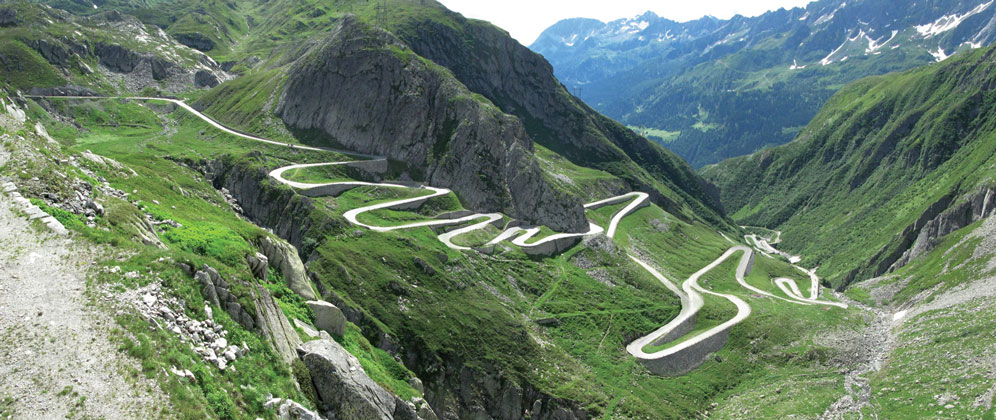
\includegraphics[width=8.5cm]{Gotthard_pass}
\vspace*{-8mm}
\caption{Gotthard Pass, Tremola}
\label{wrap-fig:Gotthard_Pass}
\vspace{-1mm}
\end{wrapfigure}
%------------------------------------------
The Gotthard pass is without any doubts not only the most important connection between northern and southern Europe, but it's also the one with the most history. During the time of the Ancient Romans, the Gotthard pass was used to connect the various cities of the empire together. The Tremola road was built around 1200 AD to facilitate communications. The Tremola was built entirely with cobblestones and is still viable today. Figure \ref{wrap-fig:Gotthard_Pass} displays these magnificent views from the Tremola. 


Nowadays, we have better alternatives to cross the Alps. The best solution is the Gotthard Road Tunnel, but unfortunately it has a restricted travel capacity. Especially in the summer months, long traffic waits can be expected before entering the 17 km tunnel; jams even longer than the length of the tunnel itself. The next best alternative is to use the new Gotthard pass, built in the 1820’s. However, differently from the tunnel that is exposed only to the usage of vehicles, this road is also exposed to the elements all year long. For this reason, during the last few years the road surface has slowly been renovated in a way to still have limited transits on the pass. This can only be done in the summer months because the winter is harsh and the pass is closed; more than 3 meters of snow usually cover the entire region. The best solution available to renovate the road was to work on one lane at the time, limiting the maximum capacity of the pass and adding traffic signals. Inevitable, waiting times to travel across the pass are to take into consideration when planning a summer trip by car. 



\subsection{Motivation}

We are interested in this project because it is a reality close to our home: we live in Ticino, on the other side of the Gotthard pass and every time we wish to visit the Swiss-German part we have to travel through the tunnel, or during the summer months we can use the pass. In the last few years the Gotthard connection between south and north has become an especially important mean of communication not only for our nation but also for Europe. 

Many projects to improve transit times have been worked on in the last few years the most important being Alptransit, which will reduce by one hour the time it takes to travel by train between Milan and Zurich in 2020. We have also recently voted to build a second tunnel to improve safety when traveling by bus and car without increasing the transit capacity. 

We hope that with this project we can simulate the fluidity on the more scenic route to cross the Alps.

\subsection{Area of study}

%------------------------------------------
\begin{wrapfigure}{h!}{10cm}
\vspace{-4mm}
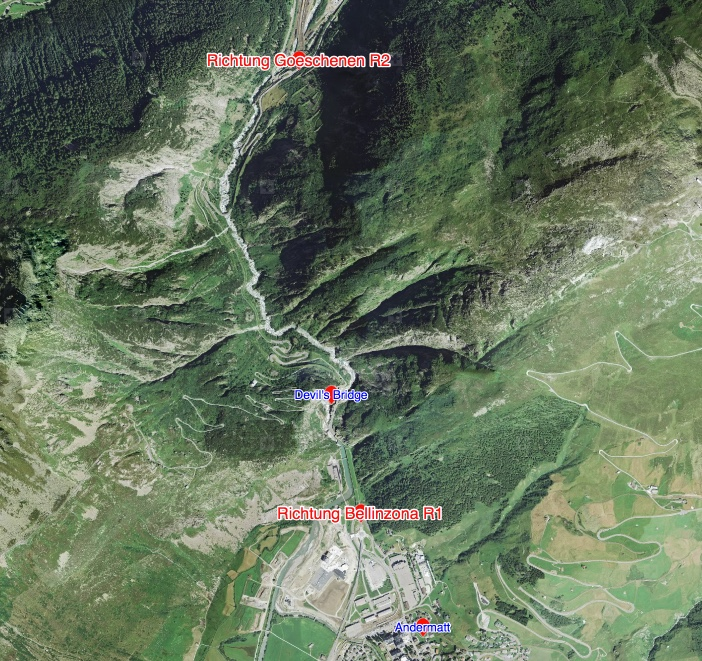
\includegraphics[width=10cm]{Map}

\caption{Satellite Map}
\label{wrap-fig:Map}
\vspace*{-3cm}
\end{wrapfigure}
%------------------------------------------

To put our simulation in a geographical perspective, Figure \ref{wrap-fig:Map} displays a satellite image of the Gotthard pass where the road work is being carried out. The pass is an important road for the people living in Andermatt. They need this stretch to move and import goods and food. The region lives on tourism, especially in the winter with ski resorts that are the primary source of income. There are also many summer hikes and places to visit like the Devil's Bridge. Considering these aspects, it couldn't simply have been closed for 3 years. Many more costs would have been involved for this renovation project from an economic standpoint. 


\vspace{3cm}






%------------------------------------------
%%%%%%%%%%%%%%%%%%%%%%%%%%%%%%%%%%%%%%%

\section{Description of the Model}

\subsection{Model Concept}

The main idea of our model came from a variation of the method used by Eric Hayoz and Janick Zwyssig in their research concluded in December 2014; \textit{``Modelling the phenomenon of congestion at Gotthard"}. They implemented the Nagel-Schreckenberg model from the 90's. The model divides the road into blocks and gives a number to each car that depends on its speed and position. 

We took this block idea and divided our road into 514 blocks. Each block is the size of an average car, 5 meters long. From here, our model creates vector blocks that it can move left and right depending on the position of a vehicle before and after a traffic signal. Cars are inserted into the simulation in a randomized order but limited by a realistic maximum number of vehicles that transit per hour given by the ASTRA datasets. 



\subsection{Situation}
Currently, the Gotthard pass has ongoing roadwork in order to renew the driving conditions and update to the new safety conditions.

As shown in Figure \ref{fig:Traffic_Situation} below (not in scale), the roadwork can be divided into several sections. Sector A, C, and E have traffic that can flow simultaneously in both directions while traffic in sectors B and D only have one lane open at any given time. This means that only one direction can flow at a time. Traffic lights in B are grouped together and green times are linked. Likewise, for the traffic lights in D. If we change the green time only for the first sector, both directions will have the same green time in that sector. If there are no cars present in the current state, the traffic light will stay red for both directions waiting for a car to be inserted into the simulation.   

\vspace {1mm}

The direction R1 represents Airolo and R2 Goeschenen. 

%------------------------------------------
\begin{figure}[h!]
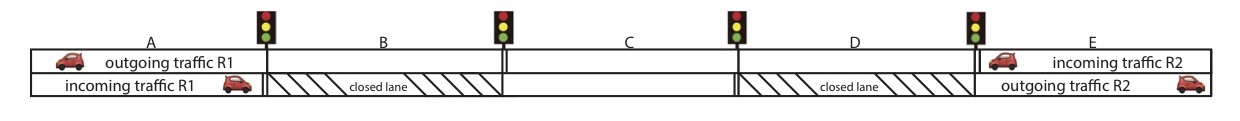
\includegraphics[scale=0.85]{Traffic_Situation}
\centering
\vspace*{-8mm}
\caption{Road Situation divided into Sectors}
\label{fig:Traffic_Situation}
\end{figure}
%------------------------------------------

\vspace{3mm}


There are however a few important facts to keep in mind:

%------------------------------------------
\begin{description}
  
  \item[$\bullet$ ] Stretch C has a maximum capacity. We therefore have to be careful not to over capacitate this sector otherwise the entire road is blocked because vehicles will not be able to flow in either direction. 
  
  \item[$\bullet$ ] If we want to reduce the average time it takes to transit this section the traffic lights need to communicate with each other and synchronize the green wave. Hence, it is important to keep both sets of traffic lights with similar green times to help the flow of traffic. 
   
\end{description}
%------------------------------------------










%------------------------------------------
%%%%%%%%%%%%%%%%%%%%%%%%%%%%%%%%%%%%%%%

\section{Implementation}


\subsection{Dataset}

We were fortunate enough to receive datasets from Astra and Swarco Traffic Switzerland. 

From Astra, we received the quantity of vehicles that passed in a given point at each given hour. They record the crossings of a vehicle divided by category. In total there are 10 categories for example cars, trucks, motorcycles, busses, campers, cyclists and many others. Naturally the highest average is contributed by cars. The dataset also tells us the direction in which the vehicles pass; R1 (Airolo) or R2 (Goeschenen). We received an Excel table with about 800.000 entries. 

From Swarco Traffic Switzerland we received the position of each traffic signal and the distances between each sector. We also received the real timing for the green and red phases.  

\subsection{Simplifications}
There are many variables that can change during the simulation and many parameters than we can vary. In order to minimize errors and facilitate the programming part of the research, we decided to simplify to our dataset and model that shouldn't impact our final results. We therefore eliminated, where possible, an implementation of differential equations and preferred constant variables. 


%------------------------------------------
\begin{description}
  
  \item[$\bullet$ ] All vehicles are considered as the same type. This implies that cars, trucks, bikes and motorcycles have the same length and speed. We can simplify this because trucks and motorcycles have opposite characteristics and average each other out. 
  
  \item[$\bullet$ ] All vehicles are approximated to have the same length equivalent to the length of one block, 5 meters. 
  
  \item[$\bullet$ ] All drivers are considered to have the same driving characteristics, meaning same speed, acceleration, and reaction times.
  
  \item[$\bullet$ ] We eliminated the different scenarios between driving uphill and downhill. Driving downhill tends to make vehicles have a higher average speed due to faster accelerations. 
  
  \item[$\bullet$ ] For each vehicle we calculated a universal average speed for the entire road work segment estimated to be 10m/s (about 36 km/h). By doing so we eliminate the need to calculate acceleration speeds and driver reaction times. 
  
 \end{description}
 %------------------------------------------
 
 
 The above cited points are the simplifications with the most impact on the outcome of the simulation. There are many other factors that we didn't consider such as weather conditions and a statistical list with tourists that don't know the road or stop for the views along their travel through the pass. The list is practically infinite and every further parameter implemented would improve, even if slightly, the final outcome of the simulation. 
  
   
  \subsubsection{Limitations}
  We have to keep in mind that our simulation is not precise with short green light times because not considering reaction times or accelerations means that for a green phase of two seconds four cars can pass. In reality we highly doubt that these many cars can legally pass although we are certain that many drivers burn the red light, especially during road works. 
   






\clearpage

%------------------------------------------
%%%%%%%%%%%%%%%%%%%%%%%%%%%%%%%%%%%%%%%

\section{Simulation Results and Discussion}
\subsection{Dataset Analysis}

Before inserting the datasets into Matlab, they first need to be prepared, selected and ordered. All this was accomplished with Excel. We decided to use the most updated and recent dataset we could get our hands onto, 2015. We first plotted the total quantity of vehicles (Figure \ref{fig:Year}) that passed each day on the pass. The data ranges from the 13th of May 2015 until the 18th of November 2015 because during the winter months the road is closed due to the snow.

%------------------------------------------
\begin{figure}[h!]
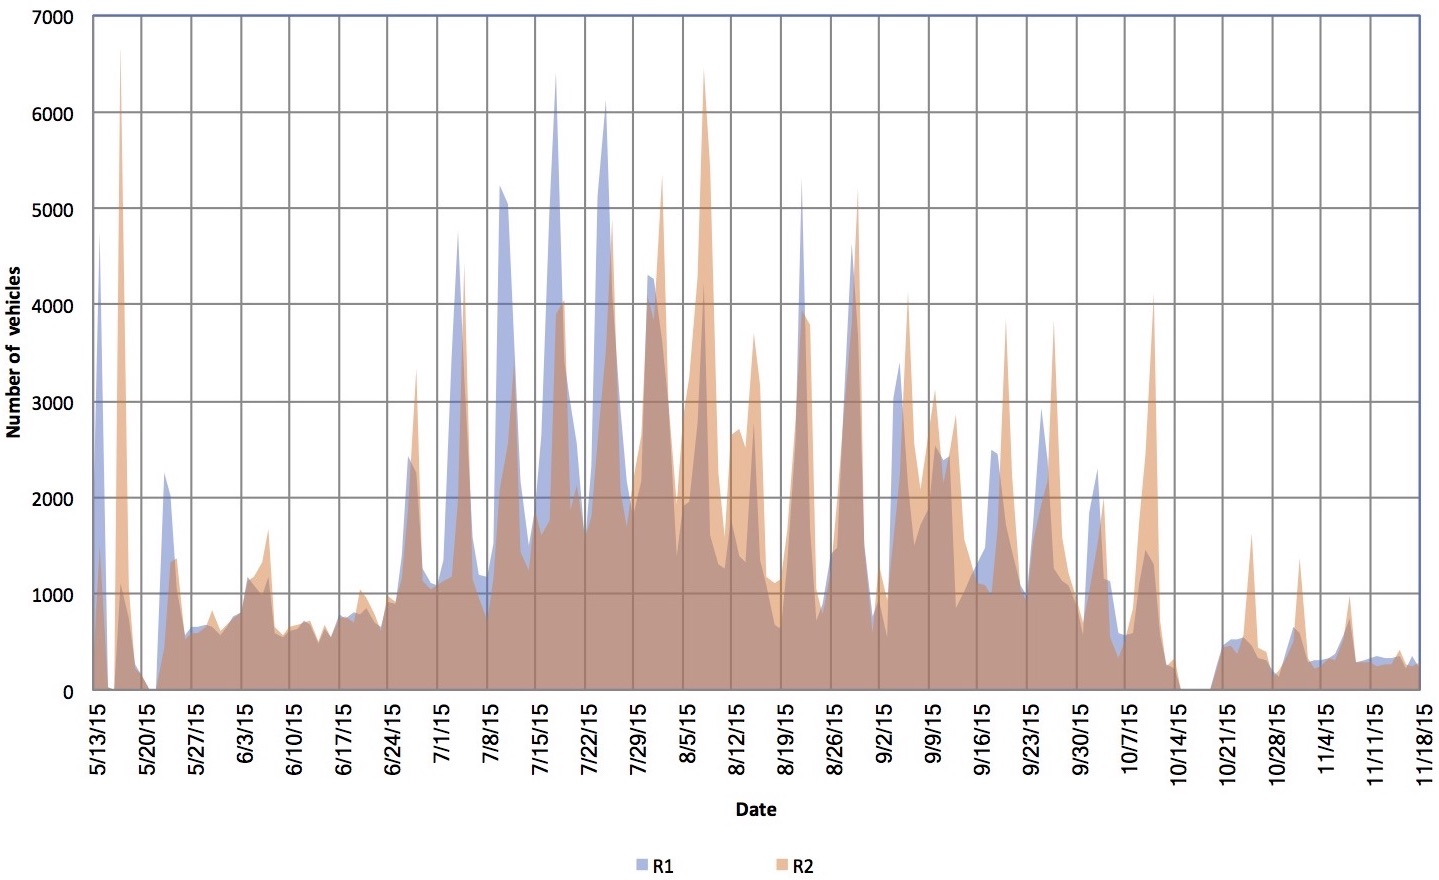
\includegraphics[scale=0.75]{Trend_Year}
\centering
\vspace*{-4mm}
\caption{Traffic per day (2015)}
\label{fig:Year}
\end{figure}
%------------------------------------------

To have an interesting result of our simulation we wanted to test the maximum stress the traffic conditions are exposed to during an extended weekend. This means when the most cars transit per hour per day. We therefore analyzed  each day and concluded that the most vehicles that traveled across the pass was during the weekend from the 31st of July to the 2nd of August.

\clearpage


%------------------------------------------ 
\begin{wrapfigure}{h!}{10.5cm}
%\vspace{5mm}
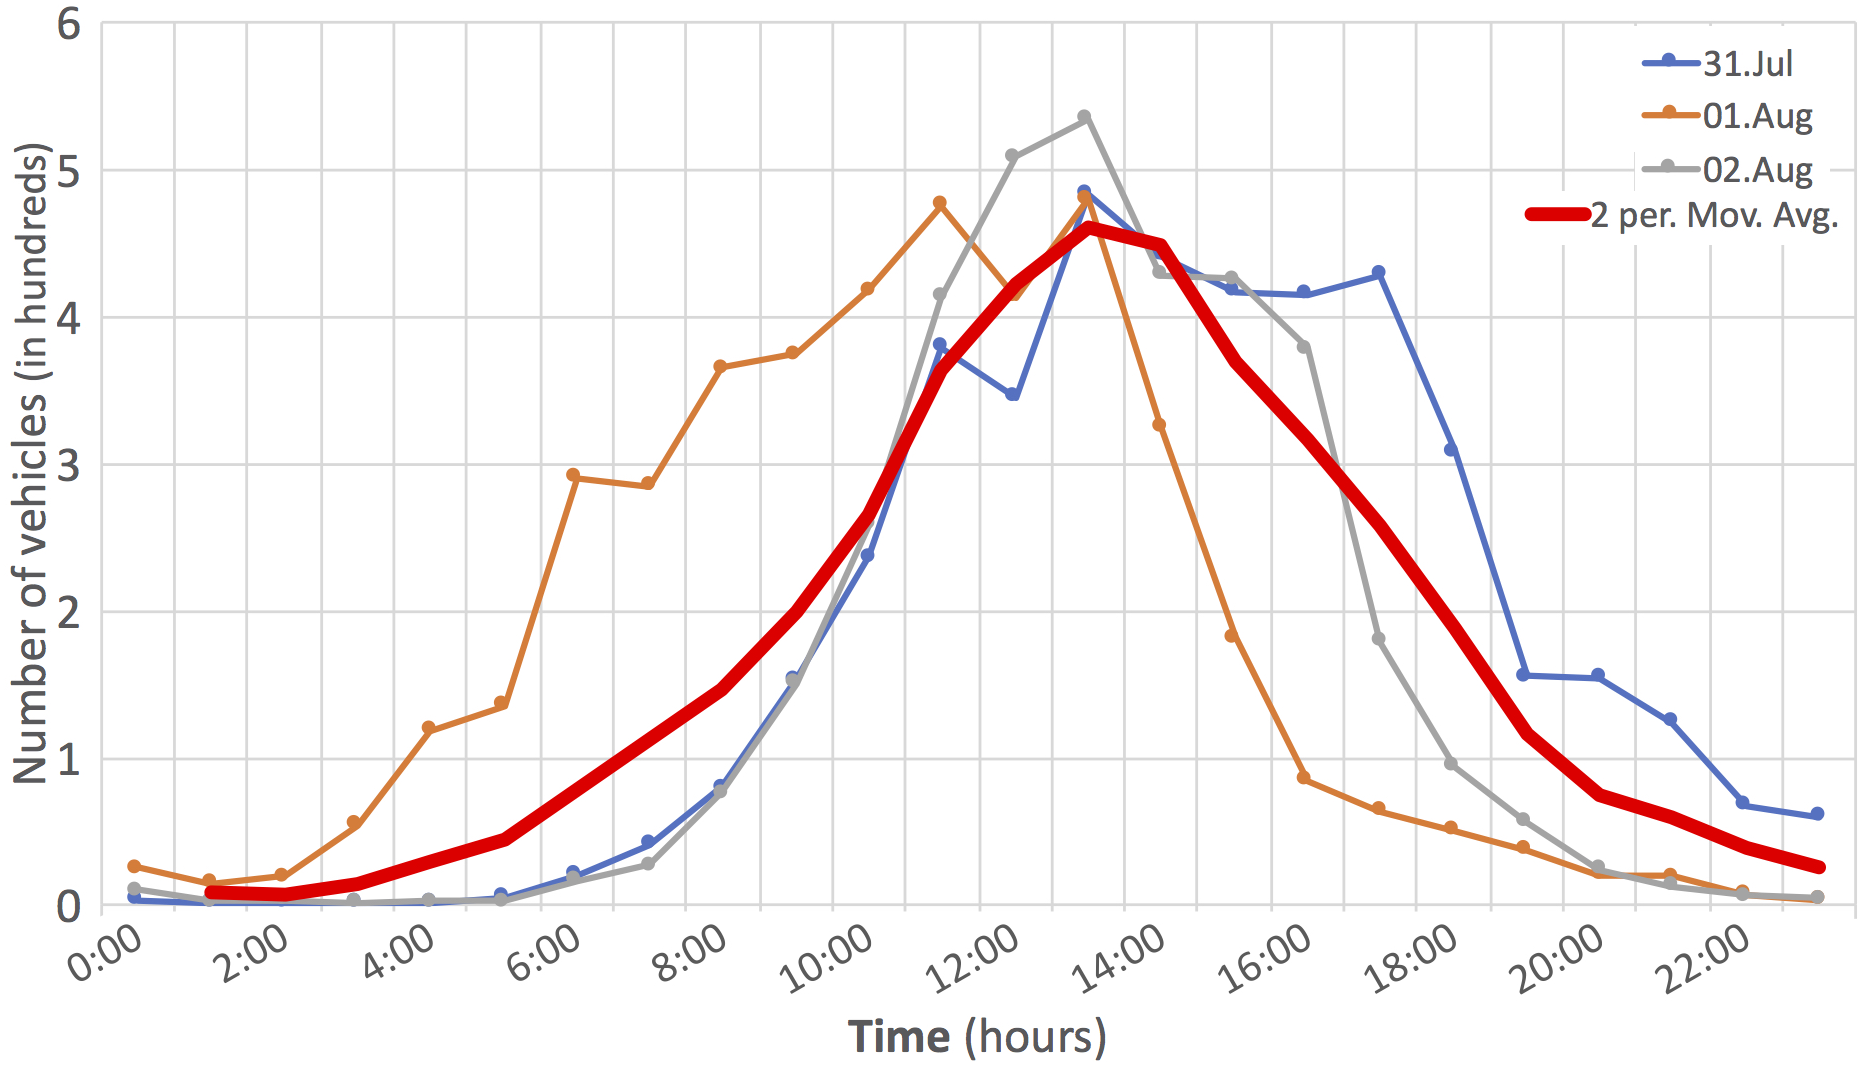
\includegraphics[width=10.5cm]{Trend_R1}
\vspace*{-8mm}
\caption{Cars per hour R1 direction (Airolo)}
\label{wrap-fig:R1}
\vspace{2.5cm}




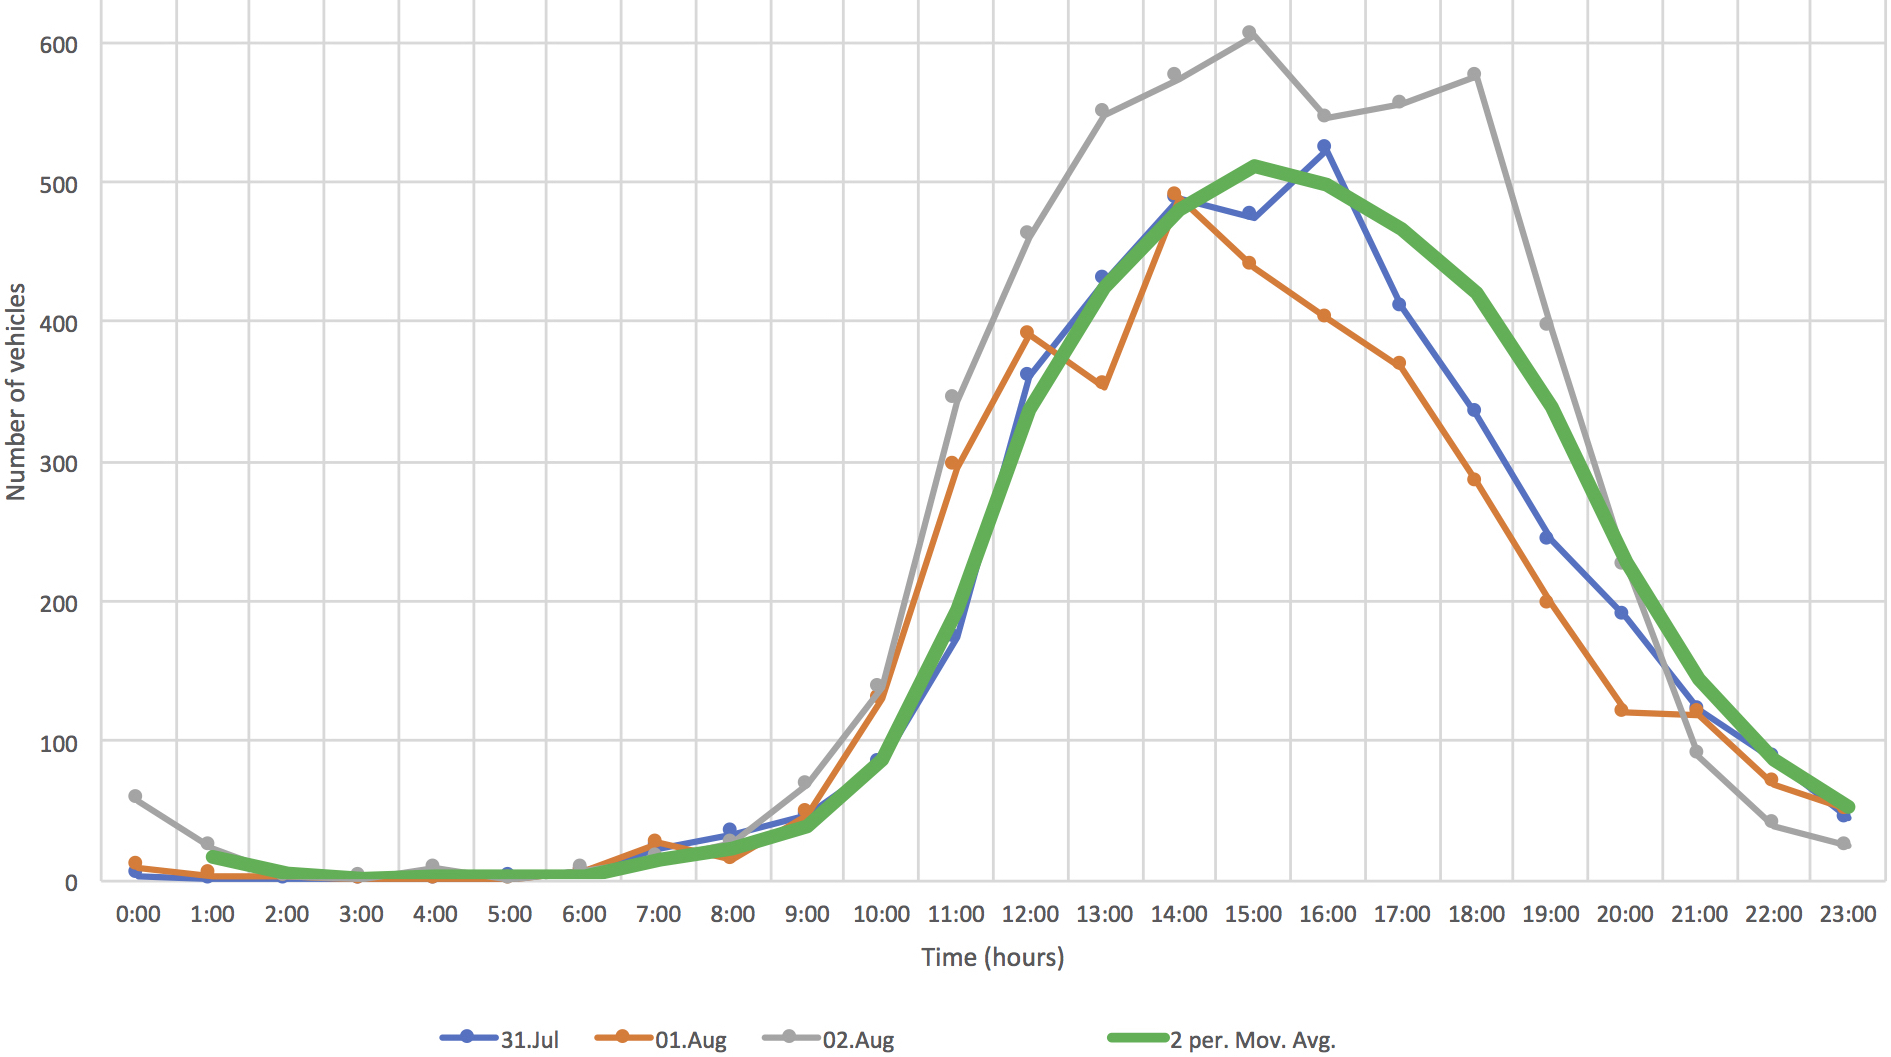
\includegraphics[width=10.5cm]{Trend_R2}
\vspace*{-8mm}
\caption{Cars per hour R2 direction (Goeschenen)}
\label{wrap-fig:R2}

\end{wrapfigure}
%------------------------------------------


We therefore subdivided our data into hourly trends. Figures \ref{wrap-fig:R1} and \ref{wrap-fig:R2} display this feature. It is interesting to note how the hourly trends and curvatures of vehicles are very similar day by day. 





The red and green trend lines display the average number of vehicles that pass for each hour during our selected time frame. Another interesting point to notice is the different habits of the population that cross the Gotthard. 



Let's start by describing people traveling to Ticino. 
\vspace{3mm}






	They tend to wake up earlier and start traveling earlier. Many Swiss-germans have summer homes in Ticino and we can assume they travel to these houses for the celebration of our National holiday. This is why they start traveling earlier, to reach their destination in time for the start of the celebration. Lugano and Locarno both have fireworks on the night of the 1st of August while Zurich omits the festivity. We can also note when the average driver stops for lunch because we see a dip in traffic. It is around 11.00 and 12.00. After lunch the curve rises again before descending constantly before night. Again, the first of August is special because of the night time festivities. 




People traveling north tend to sleep longer and travel later during the day. Traffic is a lighter during the 1st of August in the Airolo direction because of the National holiday. 

















%------------------------------------------


\subsection{Matlab Results} \label{section30_40}

After preparing the Datasets, we decided to test how well our simulation replicated the reality, in particular by overlapping the results with the time parameters that Swarco Traffic Switzerland uses to manage the road work during normal traffic. For the first traffic light, the green and red times were respectively 30 and 40 seconds. The second traffic light was 40 and 70 seconds. Fig. \ref{fig:flux30_40} displays how many cars pass per given hour though the pass but gives no information as to how long it takes them. 

Figure \ref{fig:flux30_40} also displays how the trend lines correspond with a satisfactory correlation. The main difference between the trend lines created with Excel and the Matlab simulation depends greatly on how the cars are randomly inserted in road sections. Our simulation distributes the cars with a normal distribution while the trend line uses a different statistical distribution. Another difference can be attributed to the fact that the Excel trend lines were calculated using a mean of 3 days while our simulation ran several times with the datasets of the same day (July 31st 2015). The simulation was run several times and then overlapped to show the differences that can arise caused by the randomized order in which the cars are introduced into the simulation. 
 


%------------------------------------------
\begin{figure}[h!]
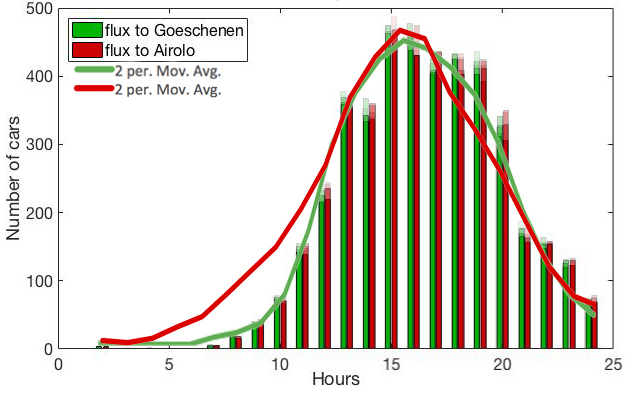
\includegraphics[scale=0.65]{ideal_timing}
\centering
\vspace*{-6mm}
\caption{Flux with official green phase}
\label{fig:flux30_40}
\end{figure}
%------------------------------------------



We will now analyze what can arise when we change the green phase time for each traffic light. The red times are fixed parameters that cannot be modified because it is the time it takes for the vehicles to empty the single lane sectors. Having a lower time could lead to head on collisions in that segment. All simulations have been run on a period of the three-day weekend but unfortunately we can only display the simulations run on the first day because the graphs do not fit on the page. We have attached in the appendix the full simulation executed during the three-day period for each traffic light parameter chosen.



\subsection{Ideal Situation}
The ideal situation is theoretically the one that corresponds to the parameters that are currently being used to manage the traffic flow. We will later verify this timing parameter. 


 As mentioned in section \ref{section30_40}, the official green phase timing for the traffic signals is 30 seconds for the first one and 40 seconds for the second. We can track each car in our simulation to display the time it takes to travel across the 2.6 km stretch. 
 
 %------------------------------------------
\begin{figure}[h!]
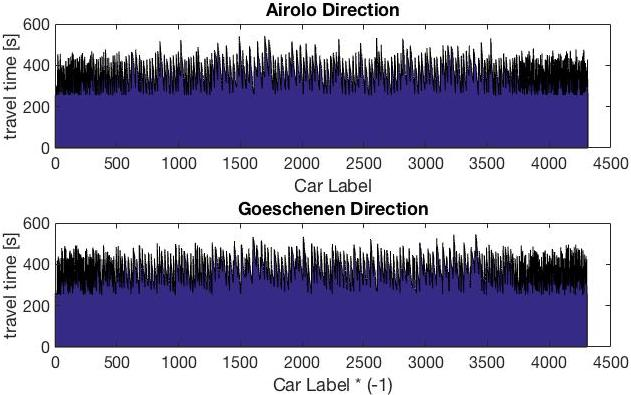
\includegraphics[scale=0.65]{travel_time_30:40}
\centering
\vspace*{-4mm}
\caption{Travel Times with official parameters}
\label{fig:traveltimes30_40}
\end{figure}
%------------------------------------------
 
 
 

The graphs in Fig. \ref{fig:traveltimes30_40} show the travel times for each vehicle inserted into the simulation. The times in both directions are similar, equivalent and regular; they vary from 260 to 550 seconds (about 4 to 9 minutes). This depends on when a driver arrives at a traffic light and if she/he is lucky to find the light that turns instantly green. The total number of cars that can travel during the interval of three days matches the total number of vehicles that transit the pass according to ASTRA data. It is about 12000 per direction. Fig. \ref{fig:flux30_40} shows how the vehicle flux is regular for both directions and is well distributed for each day. There are no significant differences between days and the maximum number of cars per hour is about 500. 







%------------------------------------------

\subsection{Limit Situations}
After testing to make sure that our simulation was valid for official times on the Gotthard pass, we decided to test different green light times to analyze what would happen to the traffic conditions. It is important to note that these parameters do not represent a realistic situation but it is important to study what happens to the system if the times are picked inappropriately and additionally it displays the mathematical limits when we tend the green light parameter to the limit situations. It is important to note we only varied one parameter, the green phase light at both traffic signals. 


%------------------------------------------
\subsubsection{Short Green Phase Times}
The first parameter settings we decided to test was to choose a short time for both sectors, in particular two seconds for the first traffic light and three for the second. 






In Fig. \ref{fig:traveltimes2_3} travel times grow linearly in both directions. Because both lights have short green times, they are very similar in form. The differences are caused firstly from the randomized creation of the cars and secondly and most importantly from the 2 to 3 ratio that occurs between the two traffic signals. This relationship allows for the road pass to allow all cars to travel without creating collisions in the single lane segments. It is interesting to notice how only the first 50-70 cars of the day can transit in a uniform way, this because the cars are very spread out. They are scattered in a very long period of time, around 4 hours. When traffic starts to get intense, heavy queues rapidly build up and the time it takes to cross tends to be very high! The last car to complete stretch of road in Airolo during the 24-hour simulation takes approximately 40000 seconds to transit, or about 11 hours!

Because of the slightly favorable green phase time, more cars can transit in Goeschenen direction because more cars are allowed to pass in its first traffic light group. 






In Fig. \ref{fig:flux2_3} it is interesting to note how the maximum number of cars that can transit in Goeschenen direction is constantly between 70 and 80 cars per hour. As for the other direction, only about 40 to 50 cars can transit during the same time frame. The maximum number of cars is also influenced by the green time of both traffic lights in this case with the ratio 2 to 3. This method to bottleneck traffic flow is currently used for the Gotthard Road Tunnel, only allowing a certain number of cars through it per day. It is important to note that this is true only because our vehicles have constant acceleration. If more than 80, respectively 50 cars arrive to the traffic lights, traffic starts to build up forming very rapidly high waiting times. Even after repeated simulations, we see how the number of cars per hour is very stable. 


 %------------------------------------------
\begin{figure}[h!]
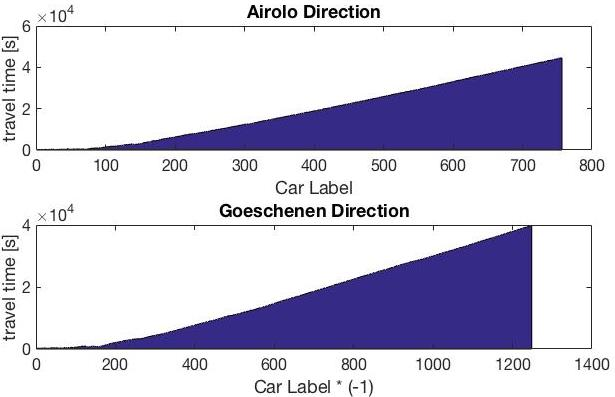
\includegraphics[scale=0.63]{traveltimes_2:3}
\centering
\vspace*{-4mm}
\caption{Travel Times with short green phase}
\label{fig:traveltimes2_3}
\end{figure}
%------------------------------------------

%------------------------------------------
\begin{figure}[h!]
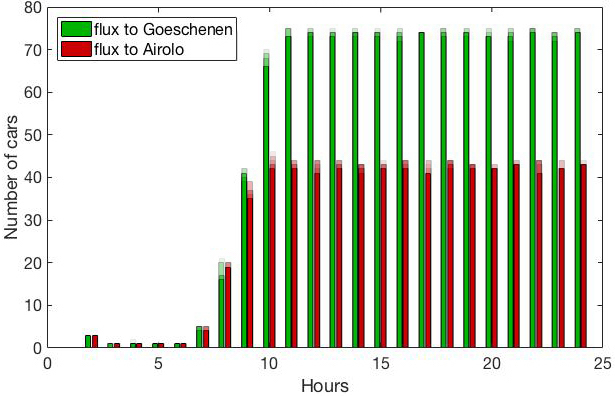
\includegraphics[scale=0.63]{shortbase2_3}
\centering
\vspace*{-4mm}
\caption{Flux with short green phase}
\label{fig:flux2_3}
\end{figure}
%------------------------------------------


\clearpage




%------------------------------------------
\subsubsection{Long Green Phase Times}

The next situation represents when both traffic lights remain green for an extended period of time, 300 seconds for the first one and 400 for the second. When heavy traffic is present in an intersection, the green phase times are higher to allow more vehicles to pass and eliminate the time of cars accelerating and the reaction times of the drivers.

 %------------------------------------------
\begin{figure}[h!]
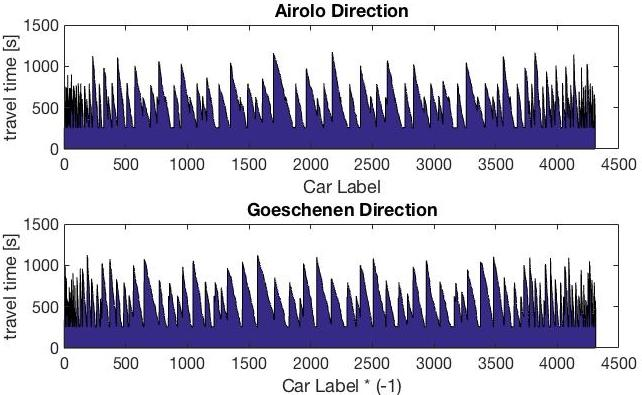
\includegraphics[scale=0.65]{longtraveltimes}
\centering
\vspace*{-4mm}
\caption{Travel Times with long green phase}
\label{fig:traveltimes300_400}
\end{figure}
%------------------------------------------

As we can visually see in Fig. \ref{fig:traveltimes300_400} the total number of cars that can transit during the simulation time of 3 days is exactly the same as the ideal green light phases. This implies that all cars can still transit the road pass as before. The difference is in the transit times. The lowest time is the same as the actual situation: this is because the driver gets lucky and upon his arrival, the traffic light is green. The highest times are reserved for the unfortunate drivers that upon arrival the traffic light has just recently turned red. We have a very high difference in transit times, from around 250 to 1300 seconds (about 4 to 21 minutes) because in addition to the normal time it takes to travel the distance, the time waiting at the red traffic light is added. 


 %------------------------------------------
\begin{figure}[h!]
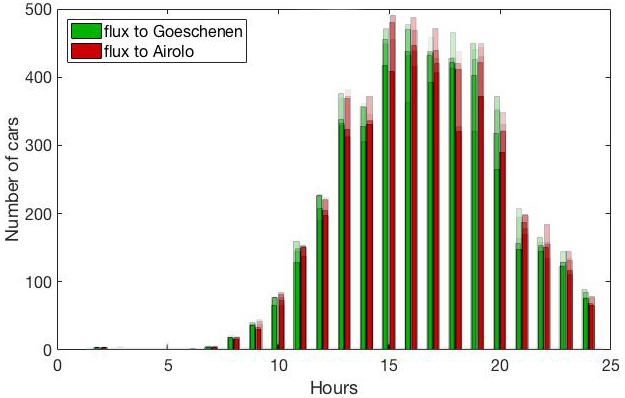
\includegraphics[scale=0.62]{longbase_300400}
\centering
\vspace*{-4mm}
\caption{Flux with long green phase}
\label{fig:flux300_400}
\end{figure}
%------------------------------------------


The flux of cars (Fig. \ref{fig:flux300_400}) in both directions is regular and well distributed during the course of the three days and there are not particular differences on a day to day basis. The cars per hour that can transit with the ASTRA datasets is exactly the same as the ideal green times but if more cars were added to the simulation, the total amount of cars that could transit is higher. 

Having high green phase times is beneficial to reduce the amount of cars building up behind the traffic lights but unfortunately increase the time it takes for drivers to transit the sectors.  





\vspace{5cm}

%------------------------------------------
\subsubsection{Combining Long and Short Green Phase times}



Taking a look at the first intermediate green phase, let's consider the situation in which the first group of traffic lights remain green for 300 seconds, while the second set for 40 seconds. In Fig. \ref{fig:traveltimes300_40} we can observe the travel times. They seem to be very similar to the situation in Fig. \ref{fig:traveltimes300_400} where the times for both traffic signals is very high. The main difference is to be found in Airolo direction. The waiting times are more equally distributed for the drivers. They all have to wait long periods of time. This is different to the Goeschenen direction in which we have drivers that wait the bare minimum while others must expect very high waiting times.

 %------------------------------------------
\begin{figure}[h!]
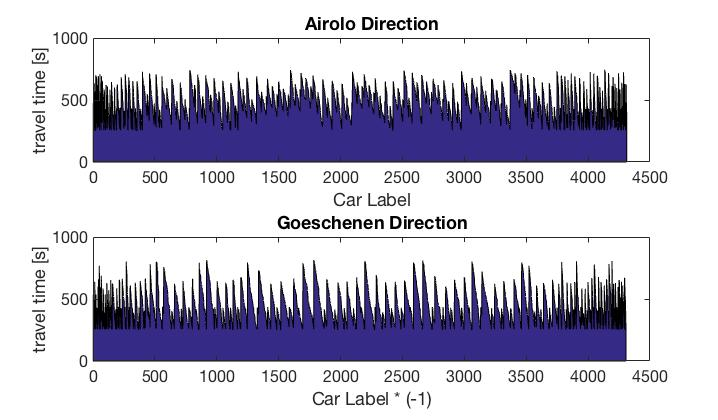
\includegraphics[scale=0.60]{traveltimeslongreal}
\centering
\vspace*{-4mm}
\caption{Travel times long and official green phase}
\label{fig:traveltimes300_40}
\end{figure}
%------------------------------------------

\clearpage

Another interesting aspect is to be noticed in Fig. \ref{fig:flux300_40}, where all cars that need to transit have the opportunity to do so, even if they have very high waiting times. We still have about 450 cars that can transit per hour. 




 %------------------------------------------
\begin{figure}[h!]
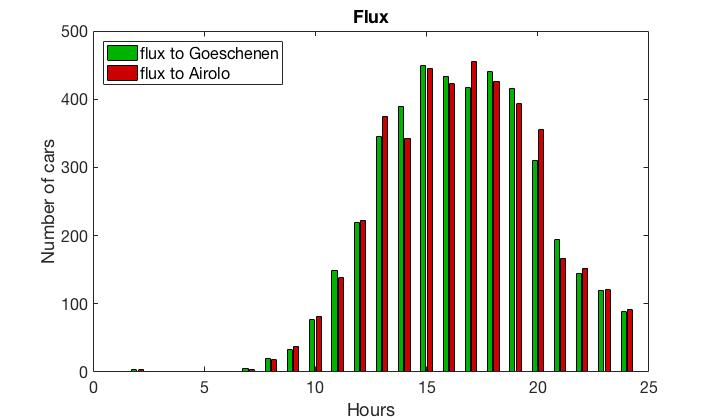
\includegraphics[scale=0.65]{fluxlongreal}
\centering
\vspace*{-4mm}
\caption{Flux with long and official green phase}
\label{fig:flux300_40}
\end{figure}
%------------------------------------------


\vspace{2cm}


Let's now analyze another mixed situation, when the first traffic signal has a 2 second green phase and the second has a 400 second green phase. This traveling apparently is very similar to the situation in which both green phases are very high and can be seen in Fig. \ref{fig:traveltimes2_40}. In both directions the travel times grow linearly and progressively but in Airolo direction we have an even heart-beating growth, it "zig-zags" its way up. This is due to the fact that the first traffic light remains green for 2 seconds, thus meaning that the difference between the waiting times of the two traffic signals is greater. Also, the standard red phase for the second traffic light is higher than the first one, resulting in this uneven growth. On the other side of the pass however, the growth is exactly like the short green phase times. The last car to transit takes almost 10'000 seconds, almost three hours. The issue with this situation is that very few cars can actually transit through the pass before the traffic condition is stalled indefinitely.






This stalling situation can be seen more clearly with Fig. \ref{fig:flux2_40}. The flux of cars to Goeschenen is blocked after around 15 hours while in the opposite direction after around 12. As mentioned above, this is because the traffic light system has cars blocked in the middle section and cannot move vehicles in either direction creating an indefinite stalling situation. In the real world this is possible and a prosegur  or police officer would manually have to free the road. The maximum number of cars that can pass per hour to Goeschenen is around 85, while it is around 50 for the other direction. 

 %------------------------------------------
\begin{figure}[h!]
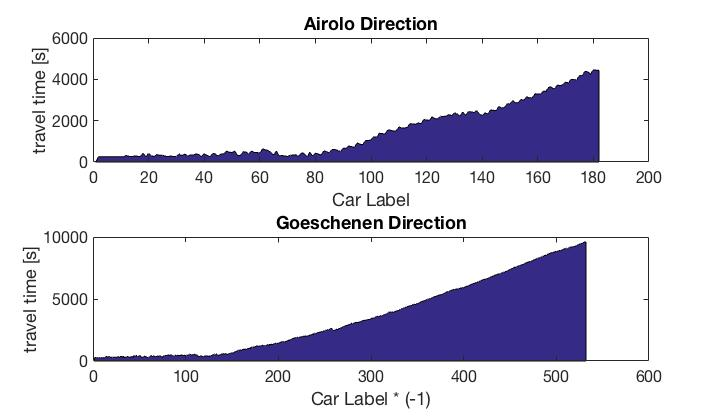
\includegraphics[scale=0.65]{traveltimesshortreal}
\centering
\vspace*{-4mm}
\caption{Travel Times with short and official green phase}
\label{fig:traveltimes2_40}
\end{figure}
%------------------------------------------
 %------------------------------------------
\begin{figure}[h!]
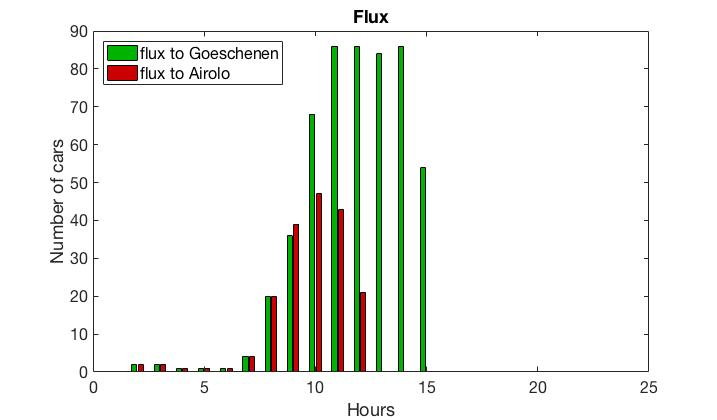
\includegraphics[scale=0.65]{fluxshortreal}
\centering
\vspace*{-4mm}
\caption{Flux with short and official green phase}
\label{fig:flux2_40}
\end{figure}
%------------------------------------------






\clearpage





%------------------------------------------
\subsection{Finding Ideal Green Phase}

We have run the simulation many times changing the green parameter by one second starting with a situation of two seconds for the first group and three for the second. With this simulation we were able to find the ideal green phase timing. We can read the ideal green time directly from the two graphs. The first time can be read on the upper graph, while the second on the lower one. The times are to be found in a certain range. We are looking for a uniform and even low travel time (in blue).  

For the first traffic light group, it is about 30 seconds, like the official parameter. For the second, it is a bit higher about 40-50 seconds, also corresponding to the official value. It is important to pick the values that allow for a margin of play. If the time were to be chosen too small and an unusually high amount of cars where to transit that day, the entire stretch could block and we would have a situation similar to Fig. \ref{fig:flux2_40}, where the cars would just jam up behind the traffic light. The black areas on the graph show the areas with a stalling situation like in the 2 seconds for the first traffic signal and 400 for the second. As we raise the value of the green time, more noise is seen in the graphs. We always have cars that can pass with short travel times, but the situation is not fair for everyone. 

The duration of the simulation is clearly visible with the two horizontal lines that divide the travel time area. These two lines are due to the fact that only a few amount of cars travel during the night hours so the travel time is not influenced.


 %------------------------------------------
\begin{figure}[h!]
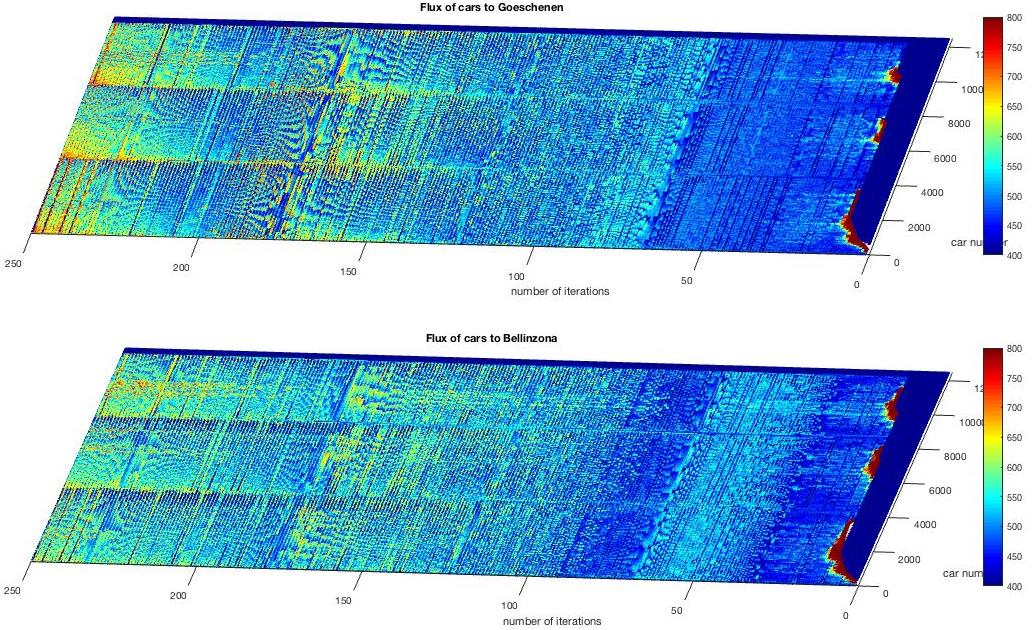
\includegraphics[scale=0.65]{3}
\centering
\vspace*{-4mm}
\caption{Travel times for changing green light parameters}
\label{fig:3}
\end{figure}
%------------------------------------------

\clearpage

It is also fundamental to verify that we have the maximum flux possible for our parameters, in order to ensure that all cars are passing with the green light parameter. We can clearly see this in Fig. \ref{fig:2}, that with a time of 30-50 seconds all cars can travel per hour for both directions. The flux is also uniformly distributed throughout the three days. 

\vspace{2cm}

 %------------------------------------------
\begin{figure}[h!]
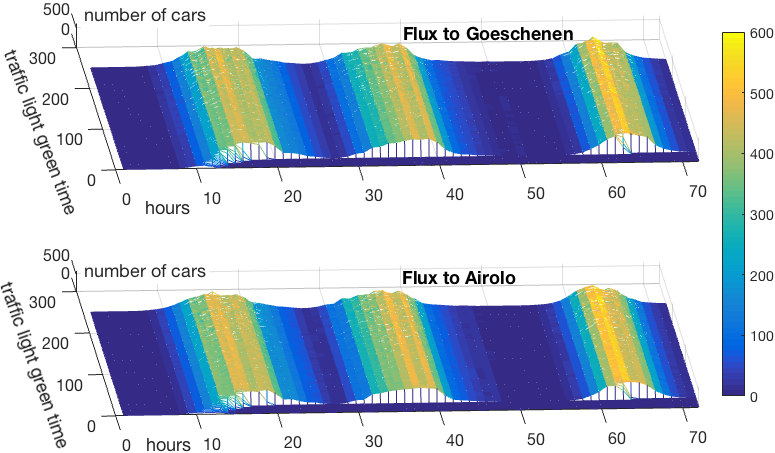
\includegraphics[scale=0.65]{fourth}
\centering
\vspace*{-4mm}
\caption{Flux for the changing green phase time}
\label{fig:2}
\end{figure}
%------------------------------------------

%\vspace{3cm}

\clearpage





%------------------------------------------
%%%%%%%%%%%%%%%%%%%%%%%%%%%%%%%%%%%%%%%

\section{Summary and Outlook}


\subsection{Conclusion}
The results of our research satisfied our expectations. We were able to create a model that represented the current situation of the Gotthard road pass. 


As we expected, fine tweaking of parameters of the green traffic time can have huge influence on how many cars can transit per hour, just like the butterfly effect. The optimal time of a green light also depends more on how many cars we are willing to allow physically to pass every time at an intersection (maximum flux and bottlenecking). 



Analyzing our data we noticed the green time always falls in a range defined by a ratio between the two traffic signals. The bottom interval is defined by the time it takes for the cars to empty the sectors that equals about 0.57 (40 seconds for the first sector and 70 for the second). The upper interval is defined by the length of these sectors that equals 0.78 (78 blocks for the first sector and 100 blocks for the second). The currently used parameters equal a 0.75 ratio (30 and 40 seconds). 


Unfortunately for our initial thesis, we were not able to find a better green phase light to transit the pass with fewer waiting times. The ideal timing is already currently being used according to our simulation with all the simplifications we did not account for. 




\subsection{Outlook}

There are always many ways to optimize a simulation. The easiest step would be to consider and implement all the simplifications that were taken to simplify the programming step of the research. We could start considering the different characteristics of drivers with regards to age, gender, and nationality.

There are an infinite amount of parameters that we could implement and each of these would make the simulation a bit more precise after every addition. Vehicle types can be further divided into sport cars, family vans and trucks. Each car has different accelerations and braking capabilities and this could affect the final result.

A further step could also be to add the driving conditions with live meteorology feeds. Fog, heavy rain, snow, hail, and sun will affect how drivers proceed along the pass and in turn this will affect the overall characteristics of a driver and the distances between the vehicles. 

Another improvement could be achieved by taking into consideration how many tourists stop along the pass or slow down to admire the panorama that this region has to offer.

Optimization is a never-ending process that at each step improves, even if by a small amount, the precision of the reality. This is why super computers are used for simulating reality because there are so many parameters that are ever-changing that need to be considered to have an accurate model that represents reality.



\vspace{5mm}

A further point of development could be to change other parameters on the Gotthard pass, like trying to tweak the distances between the traffic lights. Maybe by changing this parameter and the green light phases we could find a distance in which we can transit with lower times. This is a complicated step as the obvious best transit times would be with shorter single lane segments. We could also compare the differences between the road work with a longer single closed lane as opposed to the current situation with two single lane segments. 


As a final note, considering further parameters also needs more time to run the simulation. Our calculations already needed about four to five hours to complete on a high-end computer. This is why real simulations are run on powerful supercomputers to decrease these waiting times; especially for various business sectors that time equals money. 



\clearpage
%------------------------------------------
%%%%%%%%%%%%%%%%%%%%%%%%%%%%%%%%%%%%%%%

\section{References}
 \setlength{\parindent}{0em}
 
Images:

%------------------------------------------
\begin{description}

\item[$\bullet$ ] Figure \ref{wrap-fig:Gotthard_Pass}: http://www.wikipedia.com

\item[$\bullet$ ] Figure \ref{wrap-fig:Map}: http://www.admin.ch

\end{description}
%------------------------------------------

\vspace{5mm}

 Documentation: \par
 
 %------------------------------------------
\begin{description}
\item[$\bullet$ ] \textit 
{Modelling the phenomenon of congestion at Gotthard,
A case study} \par by Eric Hayoz and Janick Zwyssig

\end{description}
%------------------------------------------

\vspace{5mm}

 Datasets: \par
 
 
 %------------------------------------------
\begin{description}
\item[$\bullet$ ] \textit 
{ASTRA} \par 

\item[$\bullet$ ] \textit {Swarco Traffic Switzerland}
\end{description}
%------------------------------------------


\vspace{5mm}

Code: \par
 
 
 %------------------------------------------
\begin{description}
\item[$\bullet$ ] \textit 
 {List, queue, stack} written by Zhiqiang Zhang \par 
 \textit {https://ch.mathworks.com/matlabcentral/fileexchange/28922-list--queue--stack}
 

\end{description}
%------------------------------------------








\clearpage
%------------------------------------------
%%%%%%%%%%%%%%%%%%%%%%%%%%%%%%%%%%%%%%%

\section{Appendix}
In our appendix we have included the graphs from MatLab that where run on the three-day period and the full main.m MATLAB code with clarifications. 
\vspace{-1.5mm}
\subsection{Simulating Matlab results on 3 days}


\vspace{-6.5mm}

\begin{figure}[h!]
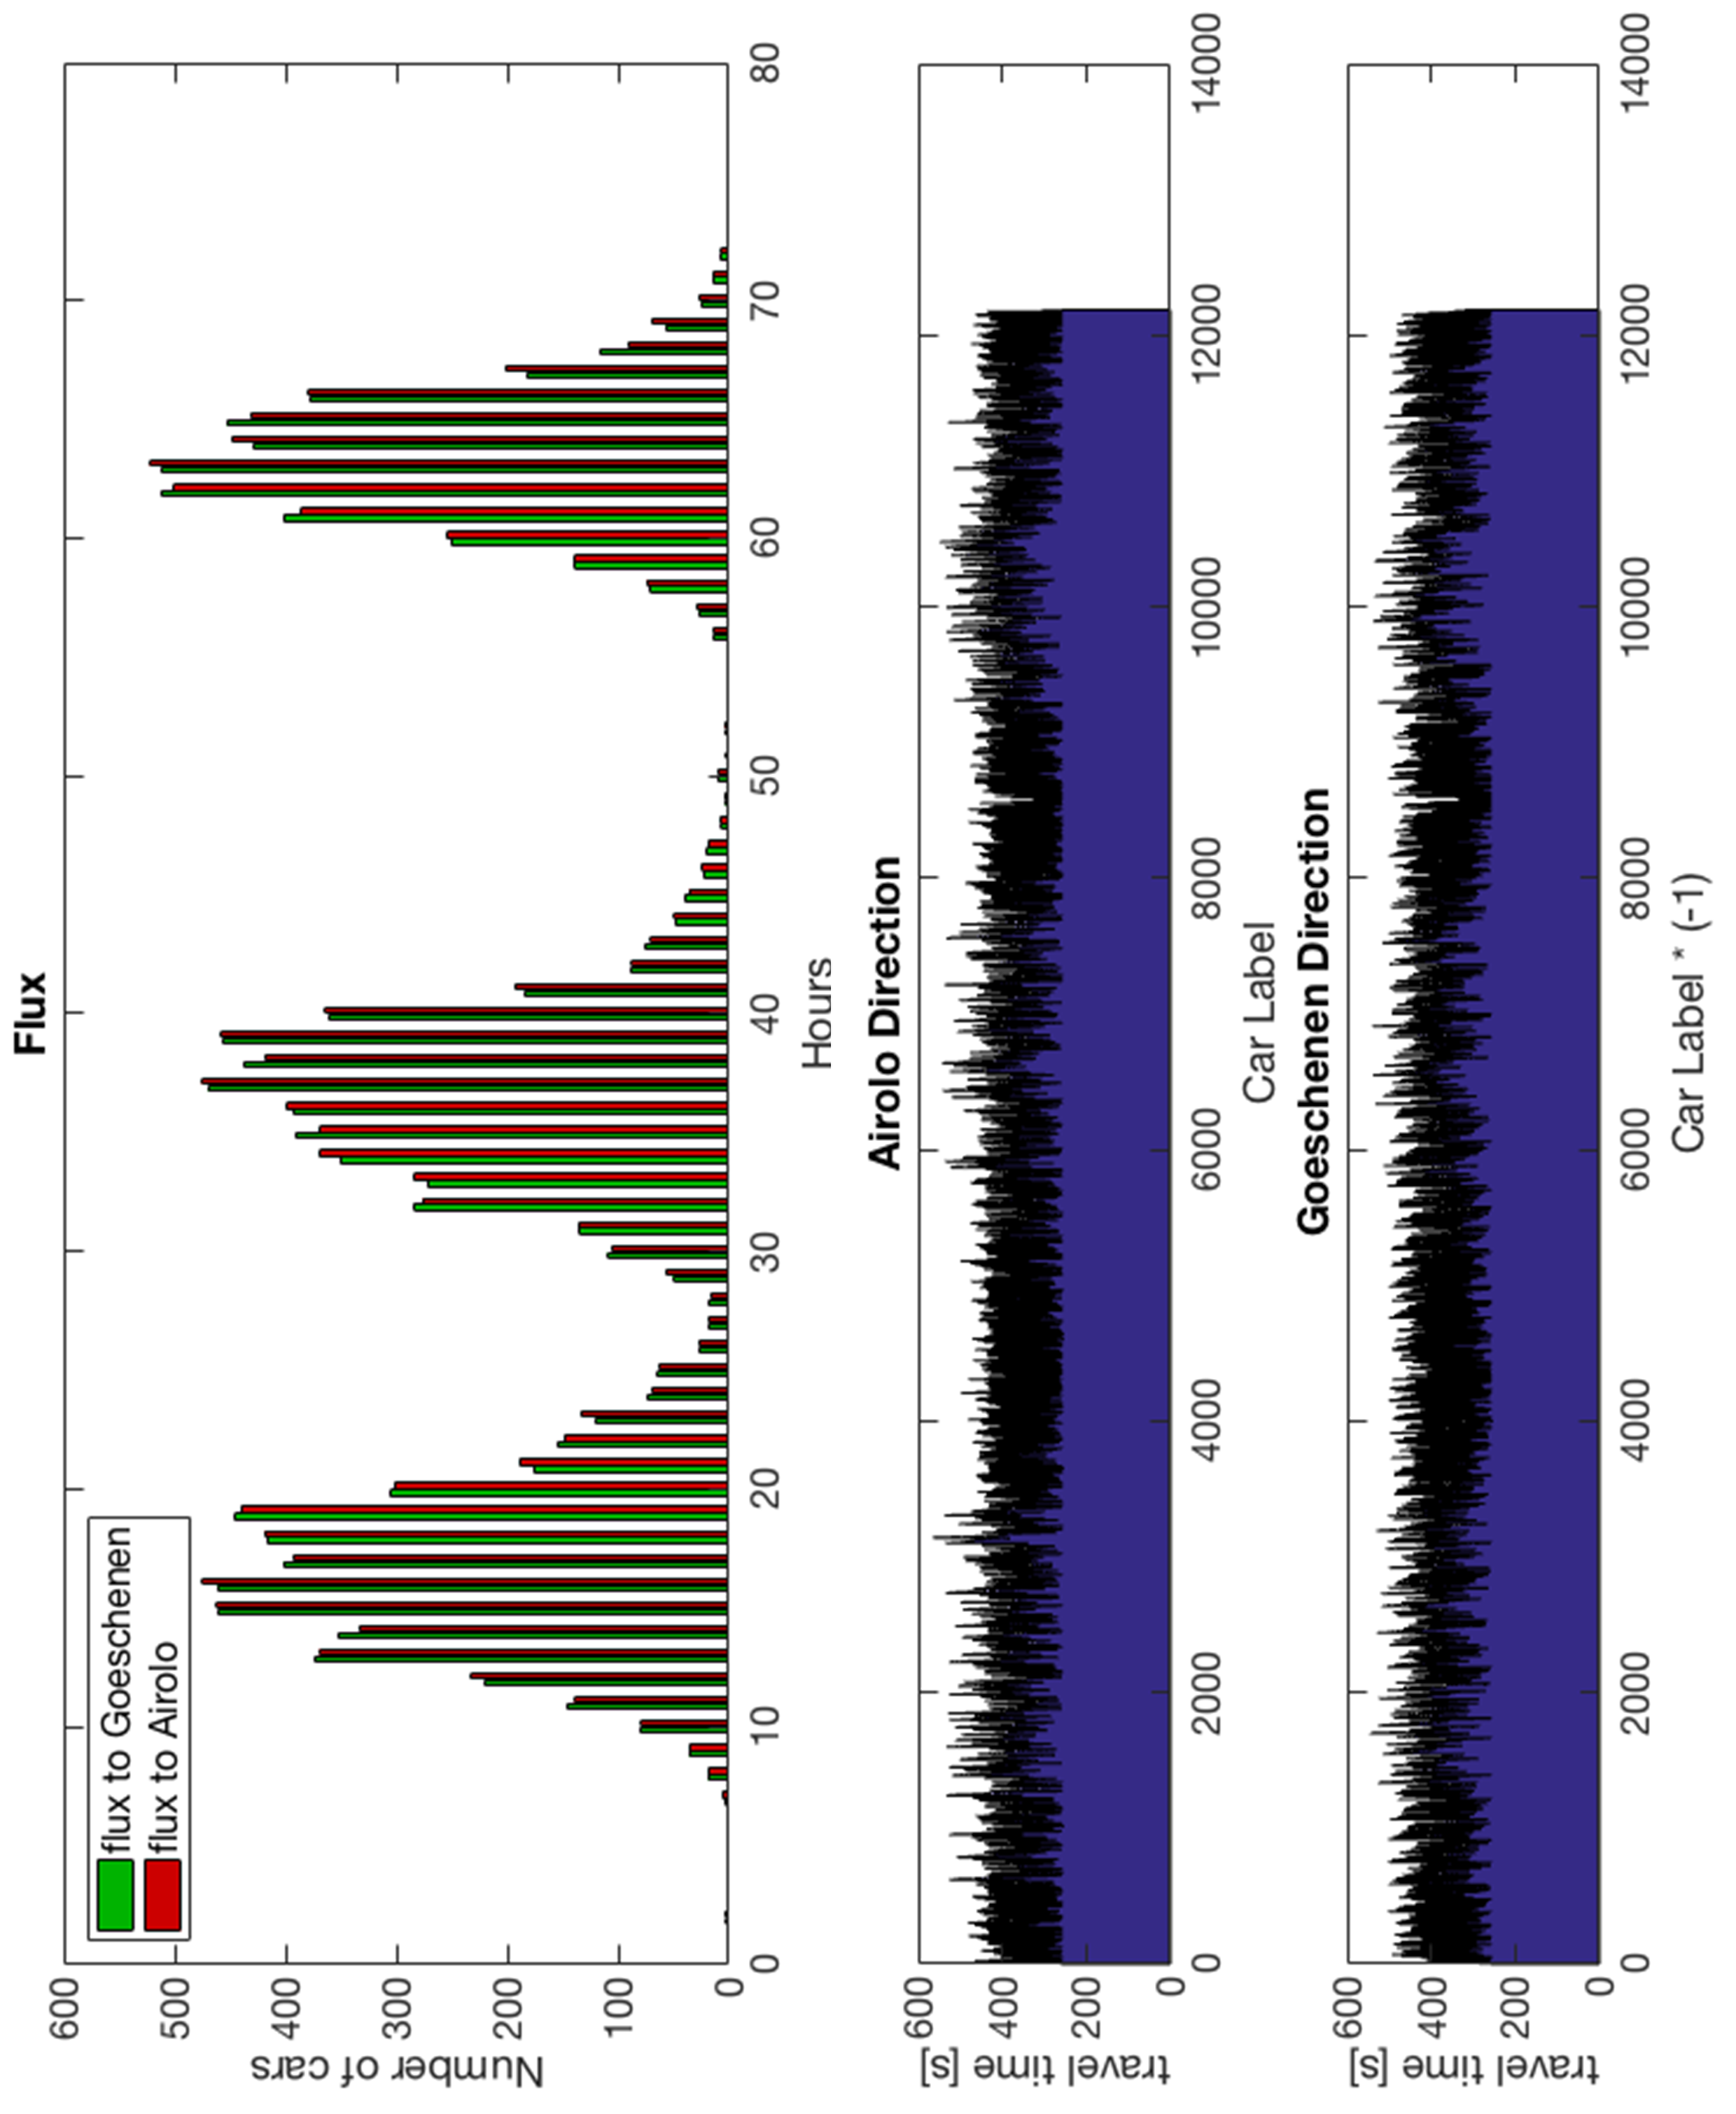
\includegraphics[scale=0.80]{30_40_3g}
\centering
\vspace*{-4mm}
\caption{30s first traffic light, 40s second traffic light}
\label{fig:30_40_3g}
\end{figure}


\begin{figure}[h!]
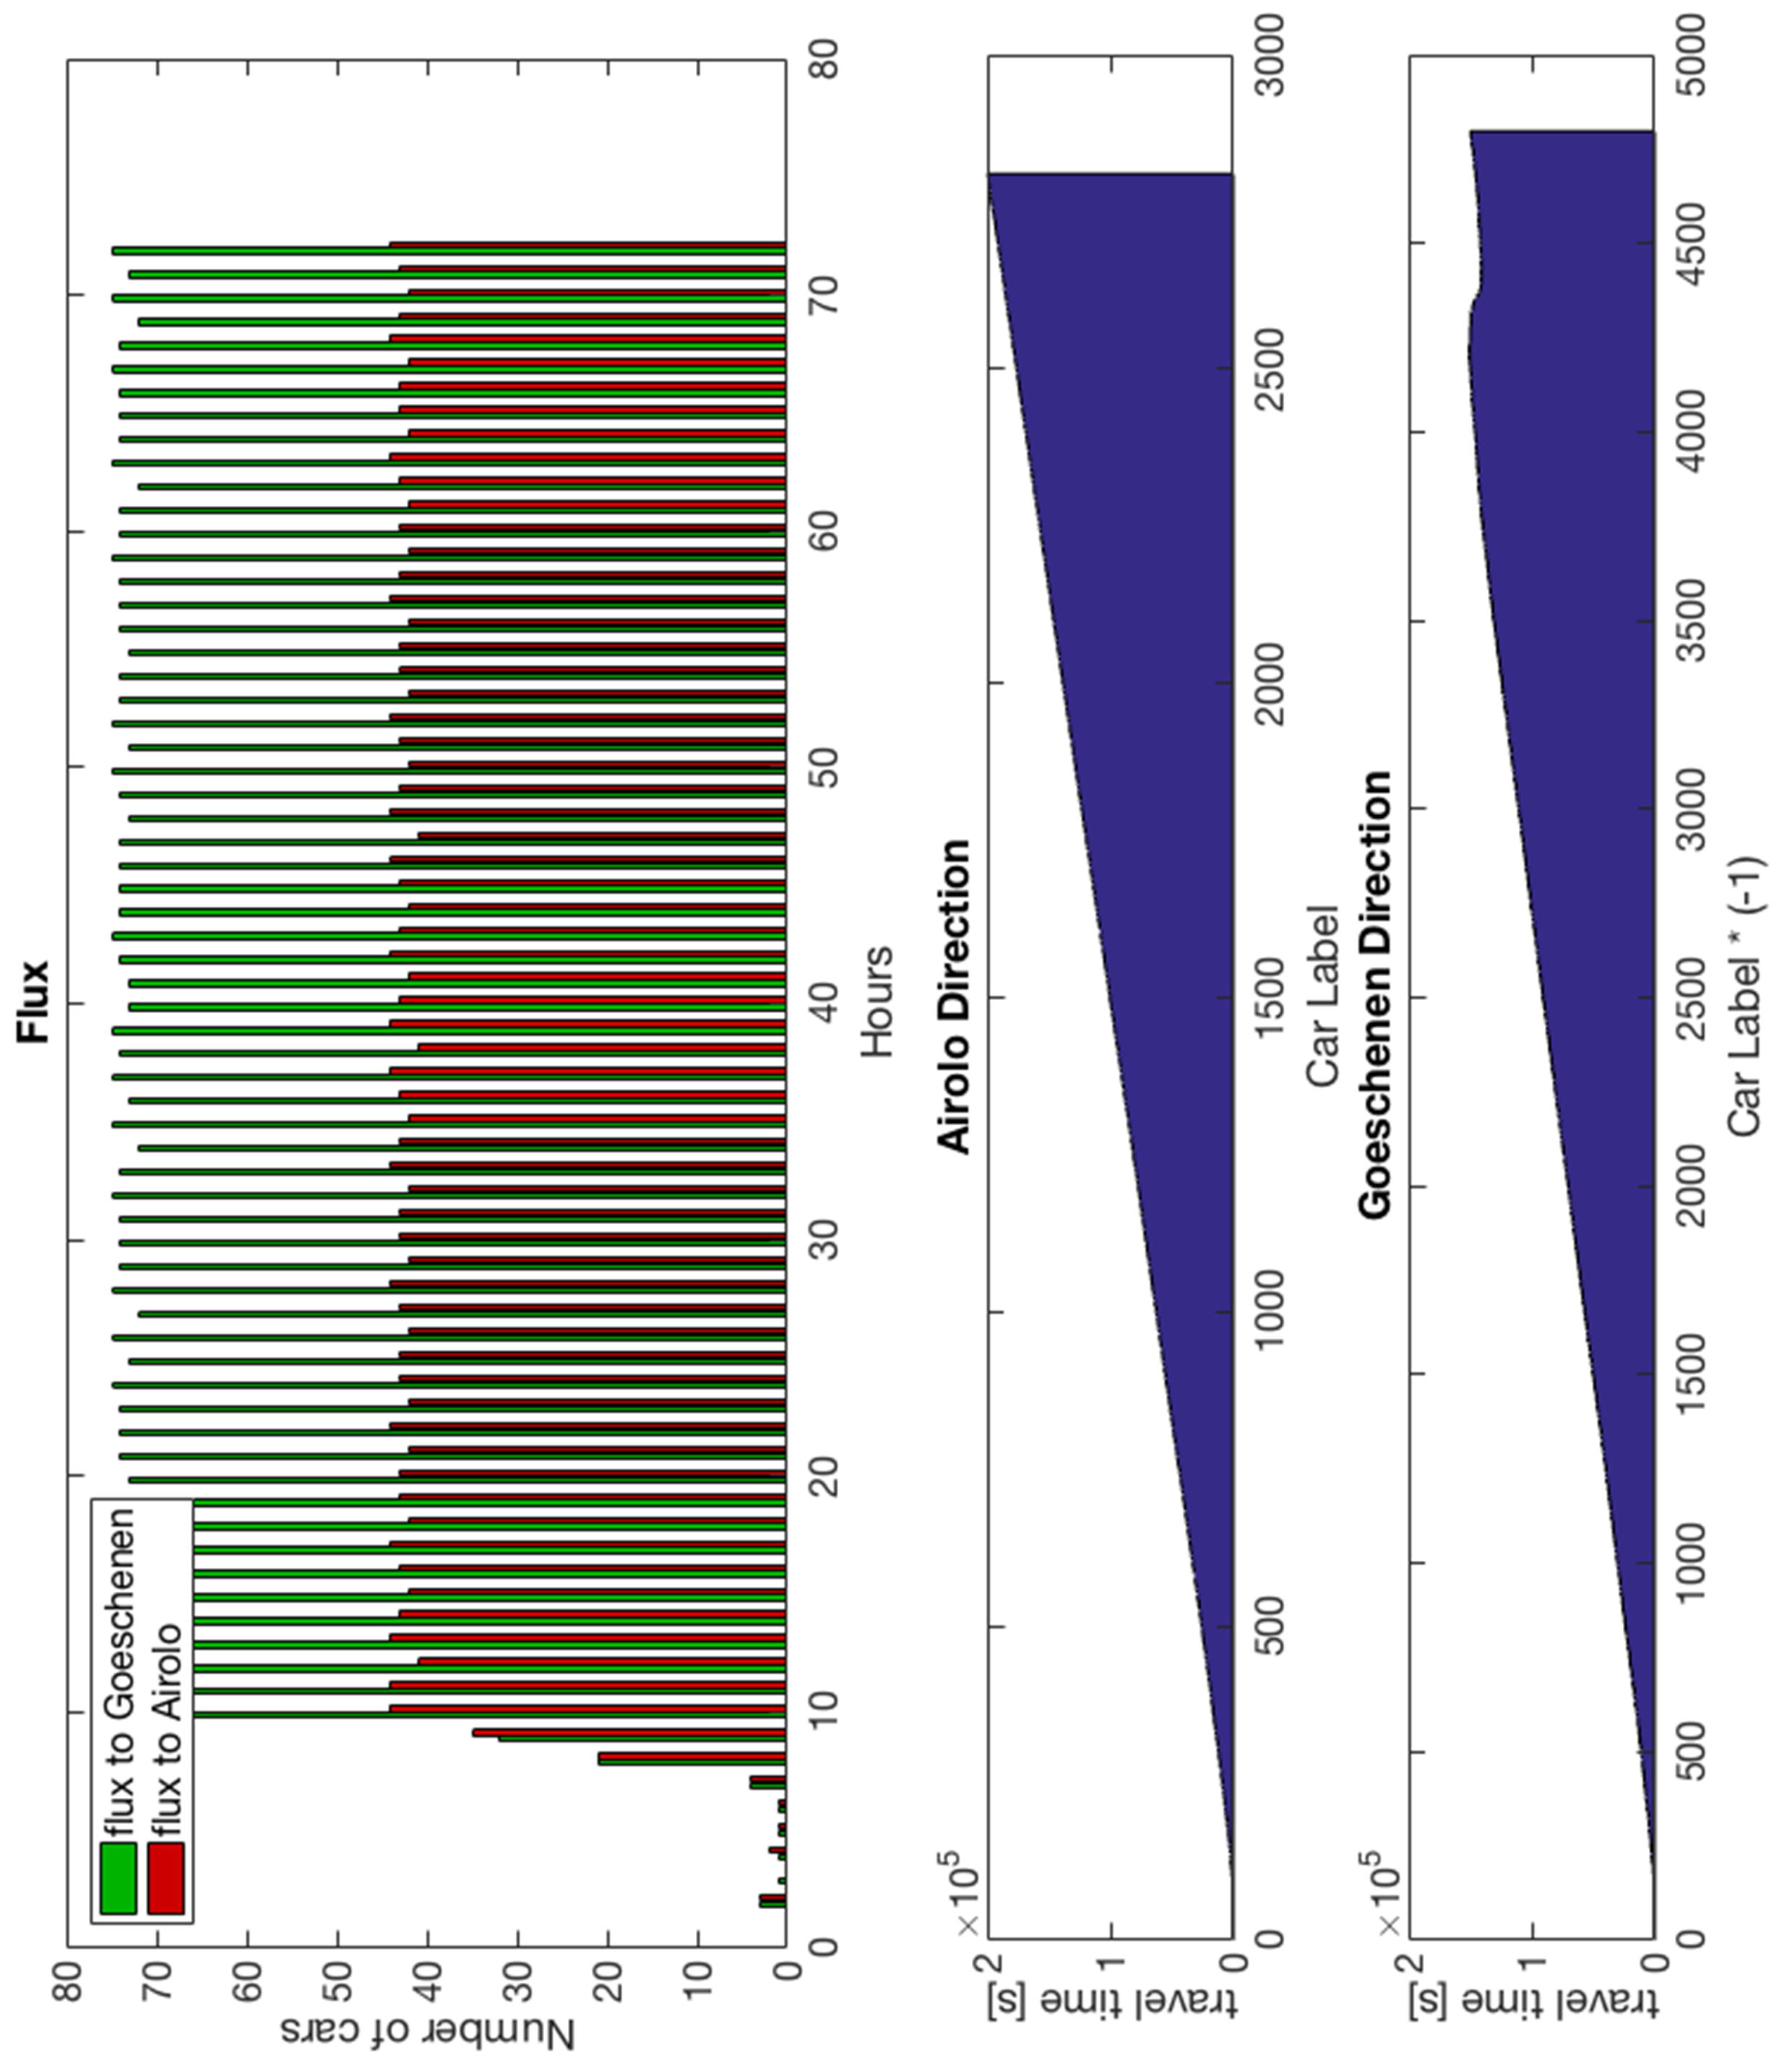
\includegraphics[scale=0.88]{2_3_3g}
\centering
\vspace*{-4mm}
\caption{2s first traffic light, 3s second traffic light}
\label{fig:2_3_3g}
\end{figure}


\begin{figure}[h!]
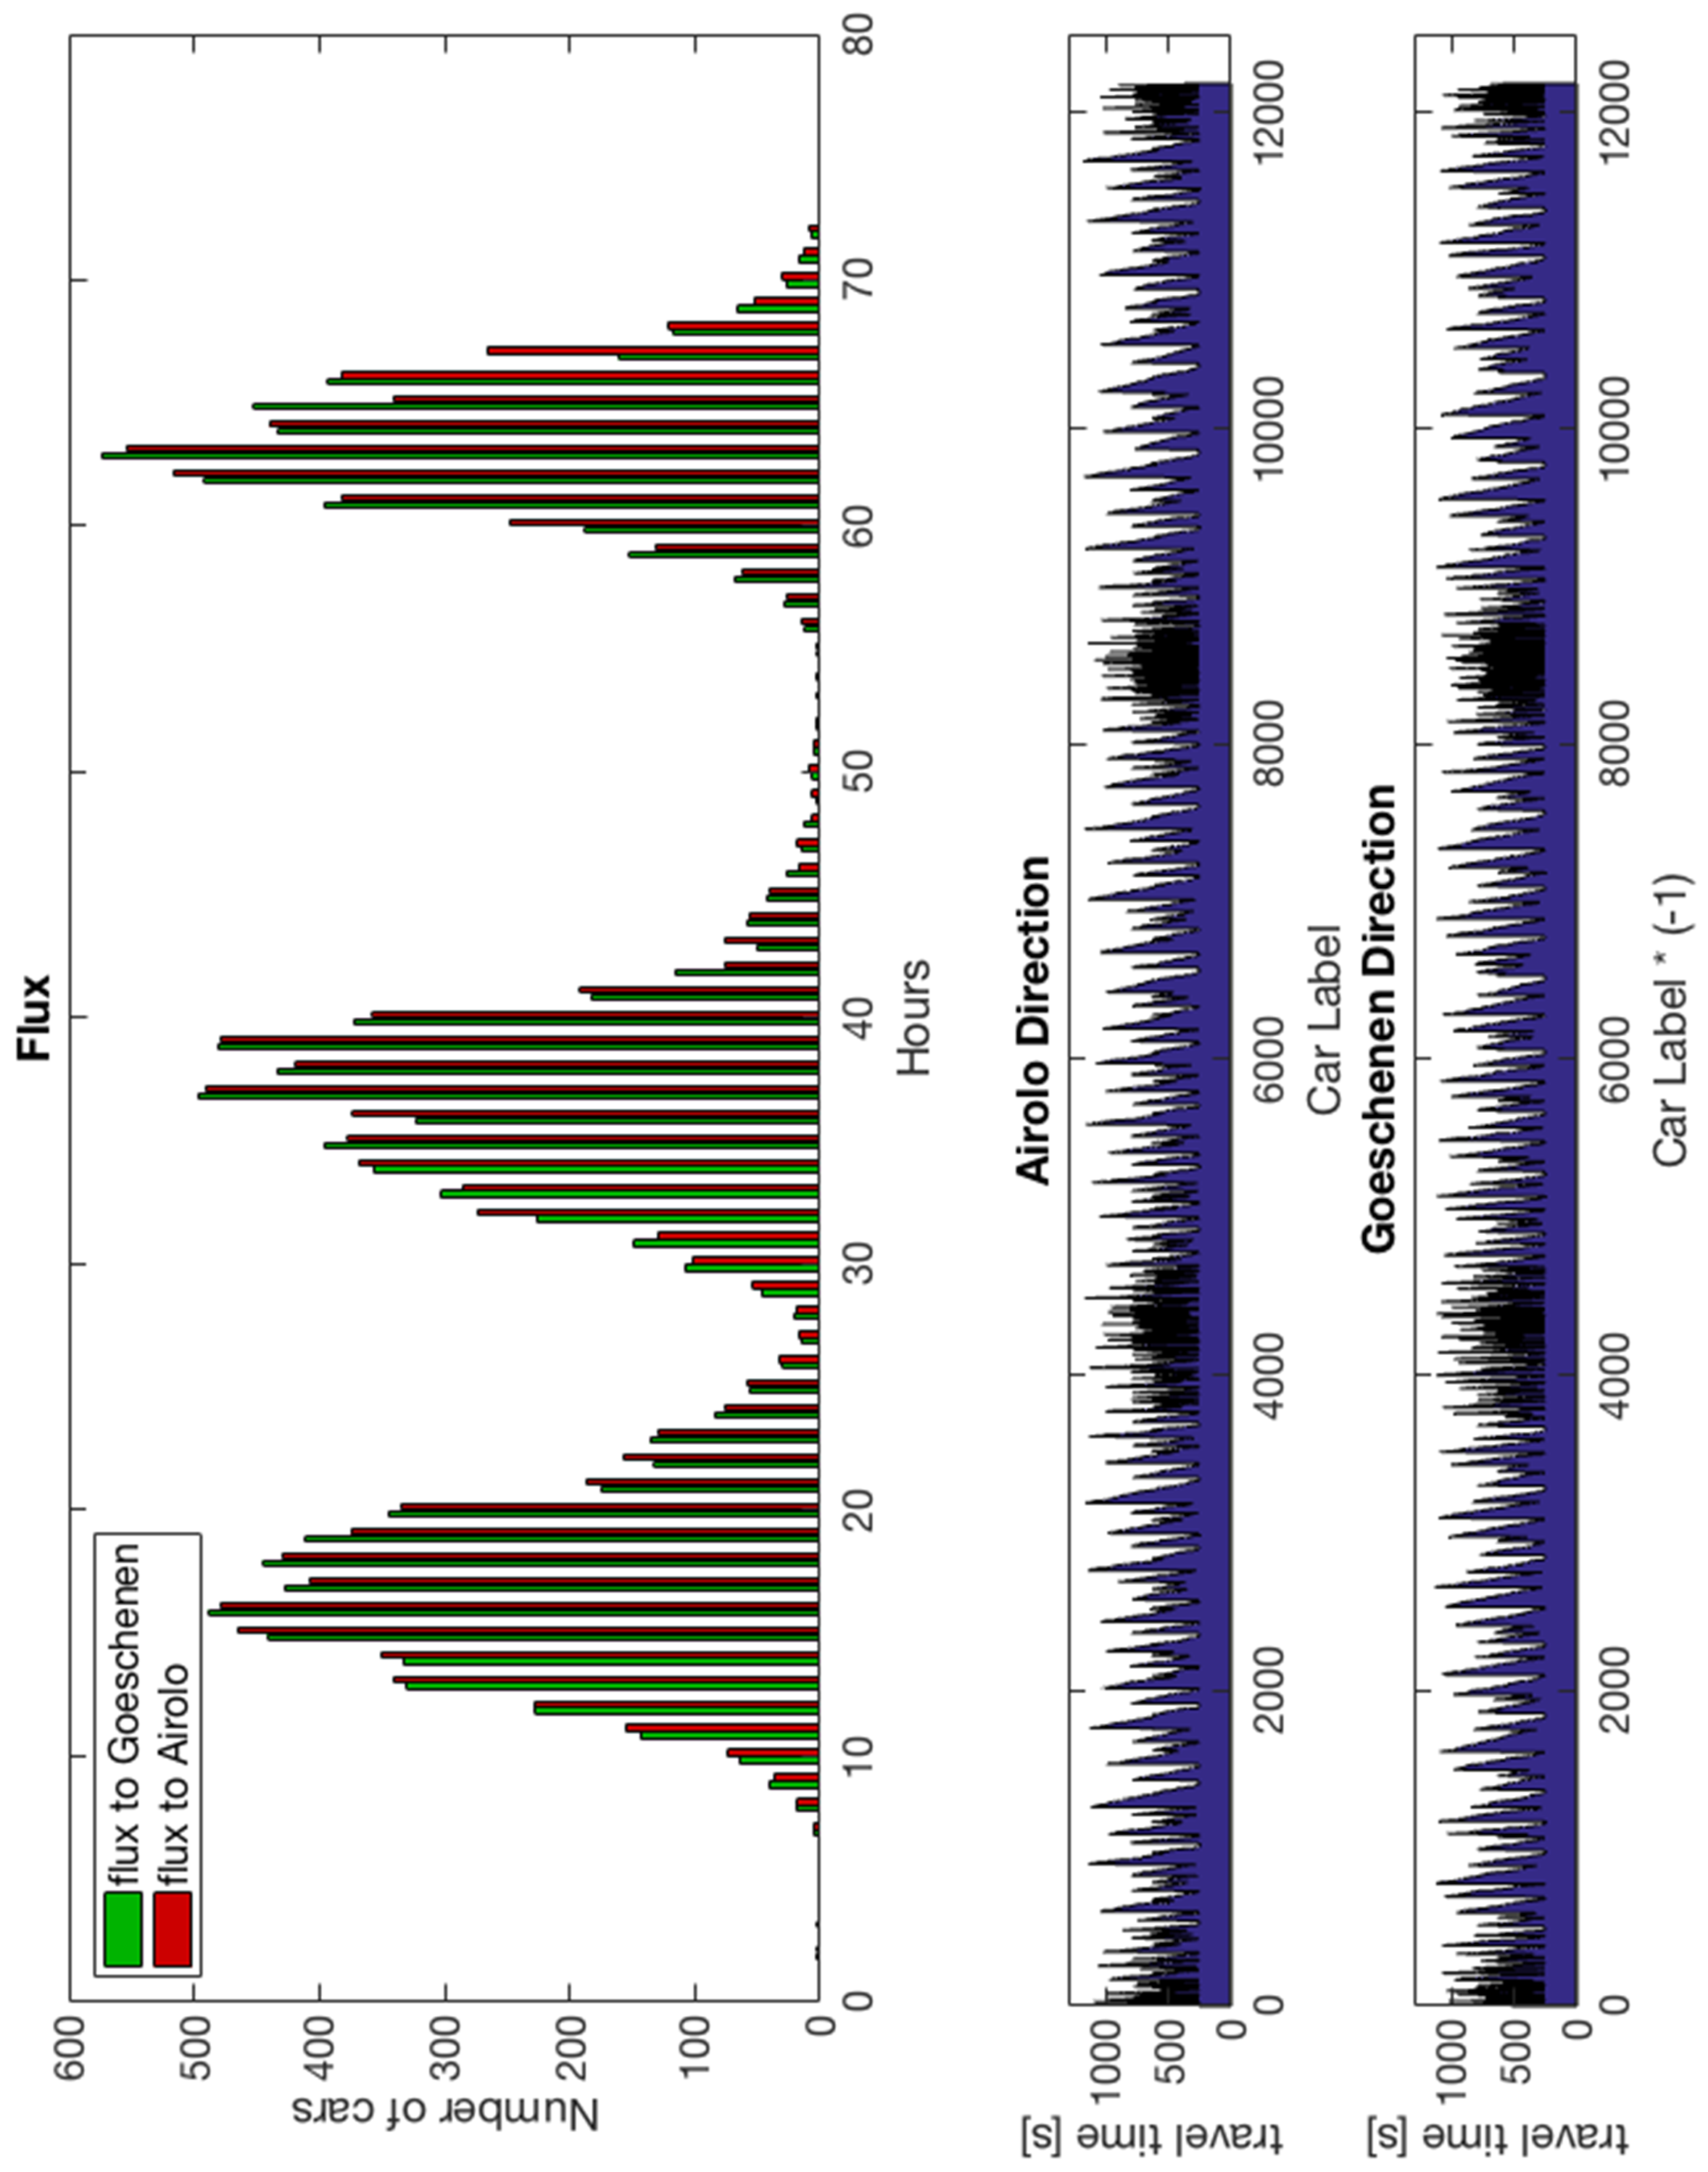
\includegraphics[scale=0.88]{300_400_3g}
\centering
\vspace*{-4mm}
\caption{300s first traffic light, 400s second traffic light}
\label{fig:300_400_3g}
\end{figure}


\begin{figure}[h!]
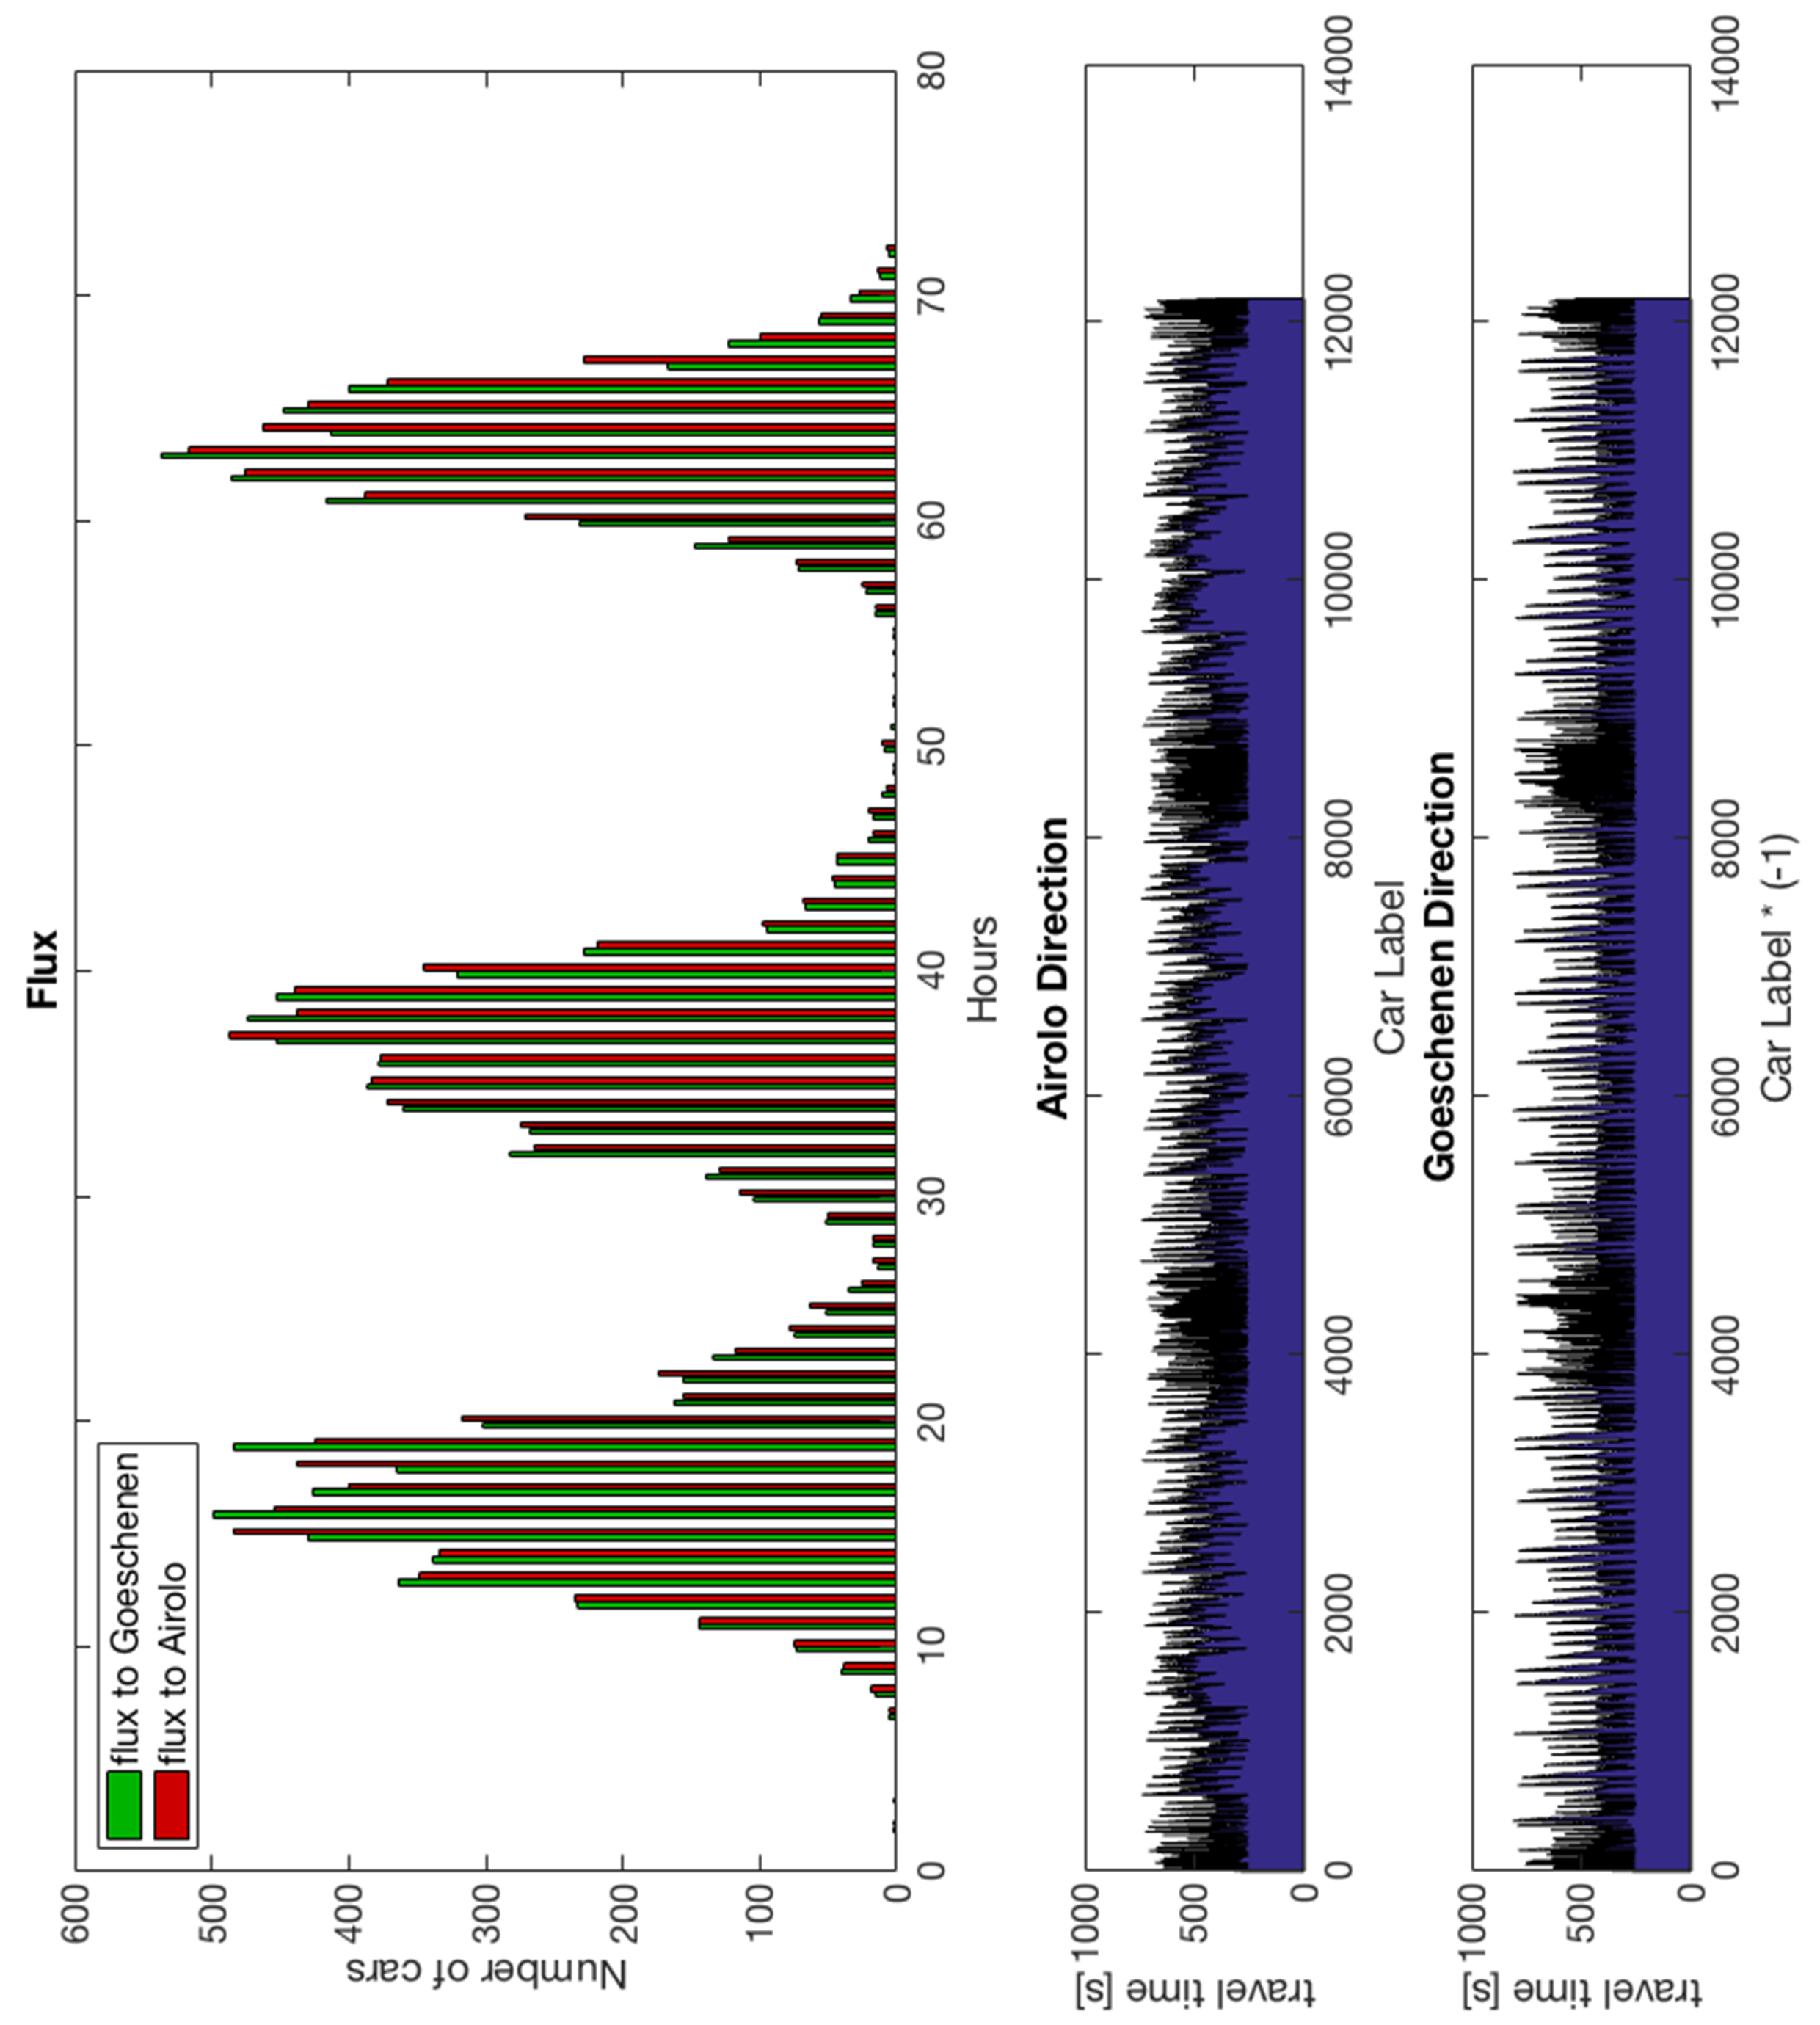
\includegraphics[scale=0.85]{300_40_3g}
\centering
\vspace*{-4mm}
\caption{300s first traffic light, 40s second traffic light}
\label{fig:300_40_3g}
\end{figure}


\begin{figure}[h!]
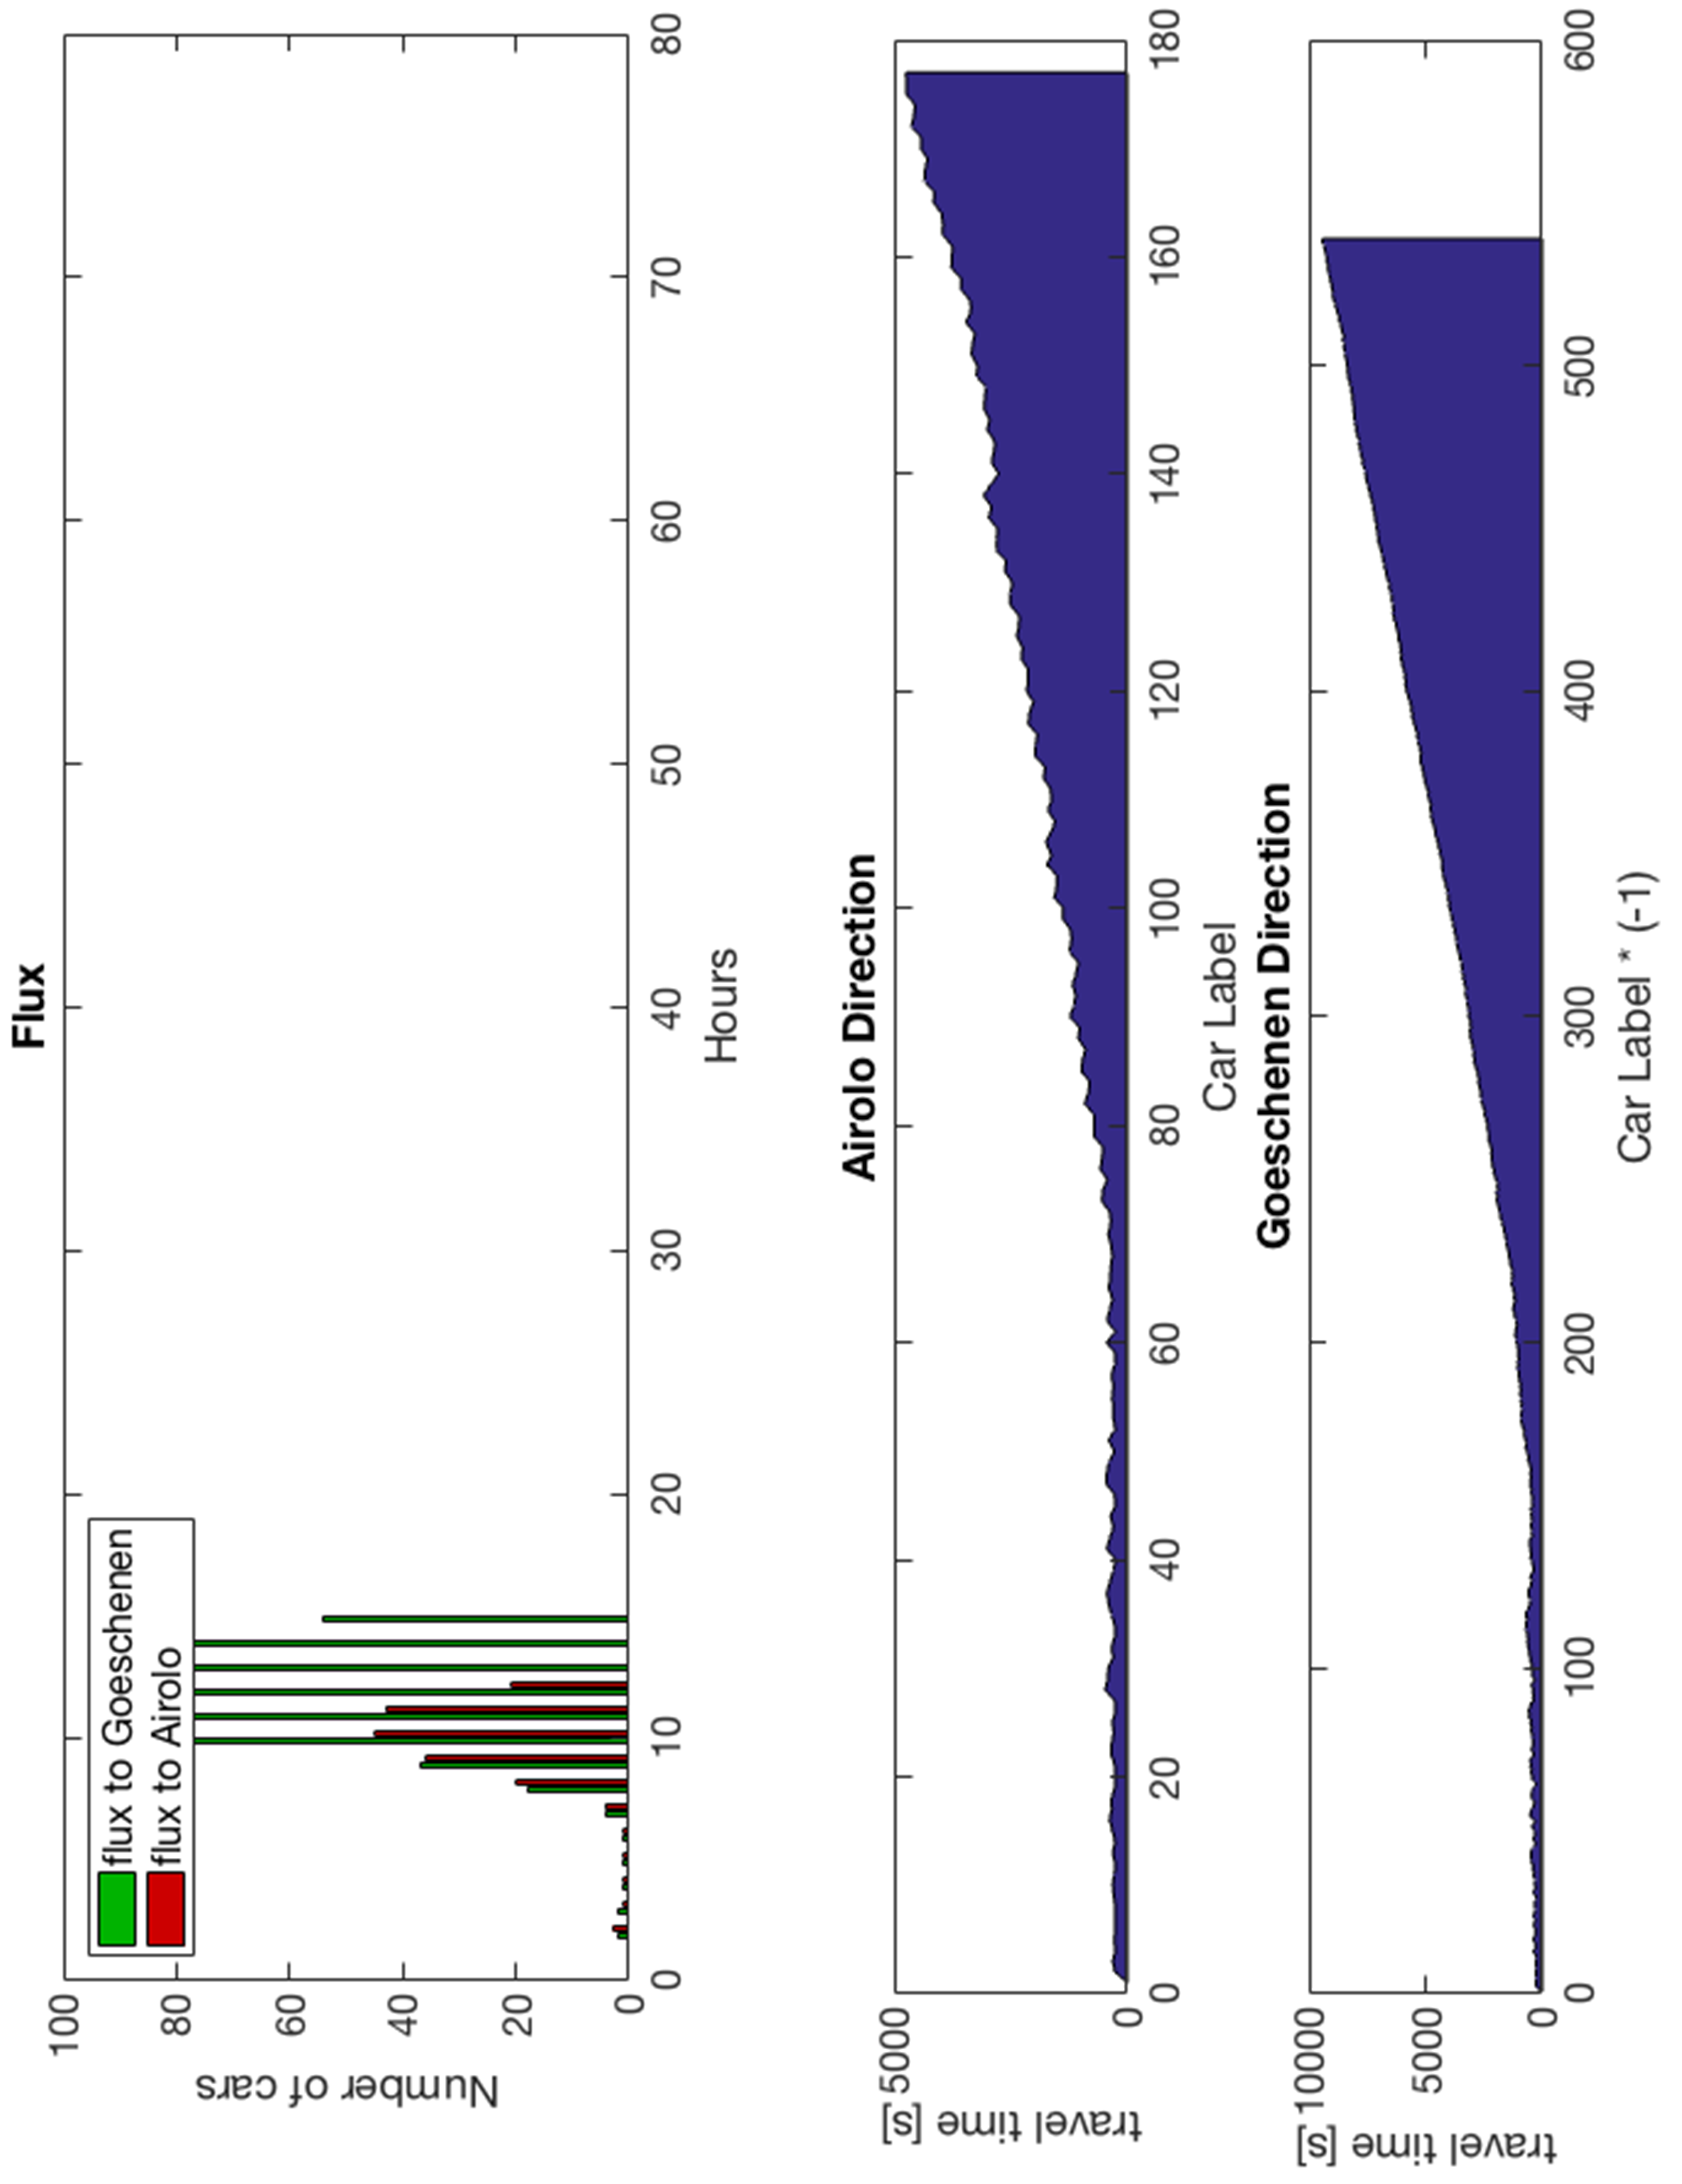
\includegraphics[scale=0.85]{2_40_3g}
\centering
\vspace*{-4mm}
\caption{2s first traffic light, 40s second traffic light}
\label{fig:2_40_3g}
\end{figure}





\clearpage
\subsection{Main.m}

%------------------------------------------
%\begin{lstlisting}
%MATLAB CODE LIST OR LIKE UNDER
%\end{lstlisting}
%------------------------------------------

\lstinputlisting{/users/davidebernardoni/Git/project_Gotthard/code/MATLAB/main.m}

\end{document}  



 
